\chapter{Classification}
\section{Classification Overview}
In the previous chapter we discussed learning a regression problem where the response was a continues value $\Yc=\R$. When the response set $\Yc$ is a finite set, this is a \textbf{classification} problem. We distinguish between classification problems where $\left|\Yc\right|=2$ (such as $\Yc=\left\{\pm 1\right\}$ or $\Yc=\left\{0,1\right\}$) and multi-classification problems where $\Yc=\left\{1,\ldots,k\right\}$. In the binary classification problem (or just "classification"), we provide a "yes"/"no" prediction. In a multi-class classification, we predict one of $k>2$ classes. For most, we restrict out discussion only to binary classification problems, though all methods below can be generalized to $k$ classes. Also, we will only deal with the Euclidean sample space $\Xc=\R^d$, namely, each sample has $d$ \textbf{features}. Therefore out setup is as follows: $ \Xc=\R^d,\Yc=\left\{\pm 1\right\} $
~\\

Throughout the chapter we discuss many different types of classifiers. For each type keep in mind the following guiding questions: (1) How does it model the classification problem? (2) What are the assumptions made on the data? (3) What is the learning principle we use? (4) How does the algorithm match the learning principle? (5) What is done in the training step and how to predict over new samples? (6) Is the model interpretable?
~\\
\paragraph{Classification Problems Examples}
\begin{itemize}
	\item Determine if a given network traffic pattern is one of a cyber attack or not.
	\item Detect fraud on credit card transactions.
	\item (Multi-class) What are the objects seen in a given picture.
\end{itemize}

\begin{example}
	Seen below are some samples of the "South Africa Heart Disease" dataset (See "Elements of Statistical Learning", section 4.4.2). Given the parameters of blood pressure, smoking, family history, etc., could we predict who has/will have coronary heart disease (chd)?
	\begin{figure}[h!]
		\centering
		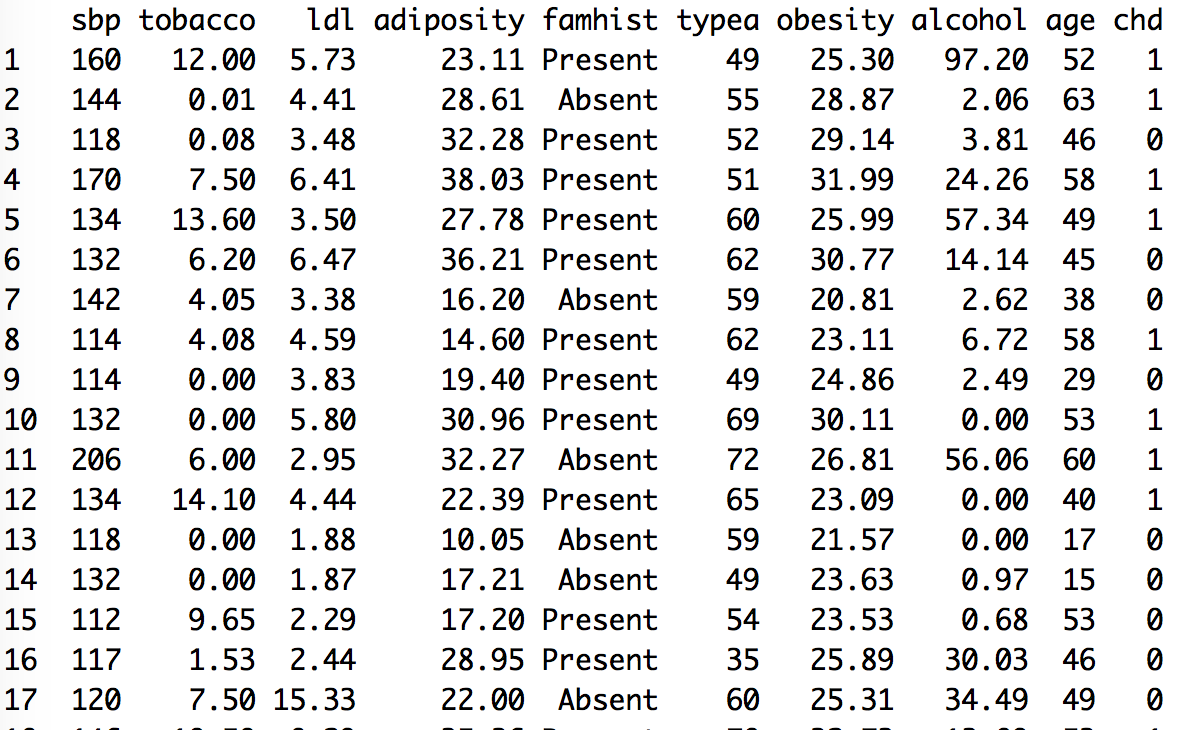
\includegraphics[width=0.4\textwidth]{chapters/classification/figures/SAheart_data.png}
		\caption{South African Heart Data from ESL}
	\end{figure}
\end{example}

\subsection{Loss Function}
When we discussed regression problems we decided to measure the performance of a given hypothesis using the square loss (and mentioned that we could also use the absolute loss). For classification problems let us consider other loss functions. A very straight forward way to evaluate the performance of a classification predictor is to simply count the number of correctly classified samples. That is, given a prediction rule $h:\Xc\rightarrow \left\{\pm 1\right\}$ and a labeled sample \trainset, the \textbf{mis-classification} loss of $h$ on this sample is:

\begin{equation}
L_S\left(h\right)\coloneqq\sum^{m}_{i=1}\mathbbm{1}\left[y_i\neq h\left(\x_i\right)\right]=\left|\left\{i|y_i\neq h\left(\x_i\right)\right\}\right|
\label{eqn:misclass_loss}
\end{equation}

\subsection{Type-I and Type-II Errors}\label{error_types}
Though many times the mis-classification loss is indeed what we are looking for, when looking closer we recognize two kinds of errors.

\begin{example}[Credit Decisions]
	Suppose we are building a classifier that predicts whether a bank customer seeking a loan is credit-worthy and will return a given loan or not. We choose the labels such that $-1$ means "not credit worth - deny loan", and $1$ means "credit worthy - approve loan". Denote $y_i$ the true label and $\widehat{y}_i$ the classifier-predicted label of sample $i$. So the two kinds of errors are:
	\begin{itemize}
		\item If $y_i=-1$ and $\widehat{y}_i=1$, the classifier predicted that a non-credit-worthy customer will return the loan. If we act on this prediction, and the customer defaults on the loan, the bank loses all the loan sum.
		\item On the other hand, if $y_i=1$ and $\widehat{y}_i=-1$, the classifier predicted that a credit-worthy customer, which would have paid the interest and returned the loan in full, is not credit-worthy and should be denied the loan. If we act on this recommendation, the bank loses the interest it would have earned on the loan.
	\end{itemize}
	Which of the two errors is more serious? Which of the two errors costs more for the bank? If we could choose which error should we avoid "at all costs" and which error could we "allow to happen", what would we choose?
\end{example}

\begin{example}[Drug safety]
	Let us look at a more extreme example to help illustrate this point. We are creating a classifier to predicts whether a certain drug \textbf{is safe} to use for a particular person, or \textbf{unsafe}/ deadly/ dangerous to use. We choose the labels such that $-1$ means "unsafe drug - do not use" and $1$ means "safe drug - ok to
	use". Similar to before our errors are:
	\begin{itemize}
		\item If $y_i=-1$ and $\widehat{y}_i$, the classifier recommends to give a drug which is actually potentially deadly.
		\item If $y_i=1$ and $\widehat{y}_i$, the classifier recommends that the patient should avoid a drug which is actually save to use.
	\end{itemize}
\end{example}

Therefore, we see that depending on the context of the classification problem, the two kinds of errors can have very different costs. We name the first error, the one we would like to avoid at all costs, the \textit{Type-I error} and the second error as \textit{Type-II error}. By choosing what label is "negative" and what label is "positive" we essentially defined what error is the Type-I error. As such, given a classification problem we try to choose the "negative" and "positive" labels such that the error we are more concern of (and therefore would like to avoid more) is the Type-I Error. That is, the error of misclassifying a negative sample by predicting it as a positive sample.

\begin{table}[h!] %TODO - align text center horizontally and vertically
\begin{center}
	\caption{Classification Error Types}
	\label{tab:error_types}
	\begin{tabular}{|c|c|c|} \hline
		\diagbox[width=3.5cm]{\textbf{Prediction}}{\textbf{Actual}} & \textbf{Negative} & \textbf{Positive} \\ \hline \hline
		\textbf{Negative}  & TN  & \vtop{\hbox{\strut\textbf{FN}} \hbox{\strut{\color{blue} Type-II Error}}} \\ \hline
		\textbf{Positive}  & \vtop{\hbox{\strut\textbf{FP}} \hbox{\strut{\color{red} Type-I Error}}} & TP \\ \hline
	\end{tabular}	
\end{center}
\end{table}

\subsection{Measurements of performance}
Once we decided what are the "positive" and "negative" labels we can device an array of performance measurements for the binary classifier. Let us consider the following template, which will help us define the four basic terms seen in table \ref{tab:error_types}:
\begin{center}
	\textit{The classifier \{truthfully/falsely\} stated \{positive/negative\}}
\end{center}

So when the classifier \textbf{truthfully} states either "positive" or "negative" we understand that this statement (i.e prediction) was correct. In this case we are looking at the \textbf{True Positives (TP)} - positive samples that were classified as positives, and the \textbf{True Negatives (TN)} - negative samples that were classified as negatives. In the case the classifier \textbf{falsely} stated either "positive" or "negative" we understand that this statement (i.e prediction) was incorrect.
\begin{itemize}
	\item If "the classifier \textit{falsely} stated \textit{positive}" we understand that the prediction was that the sample is positive, but in reality this is incorrect and therefore the true label is negative: $\widehat{y}=-1,\, y=1$. These are the \textbf{False Positives (FP)}, which by convention we decided to define as the Type-I error.
	\item If "the classifier \textit{falsely} stated \textit{negative}" we understand that the prediction was that the sample is negative, but in reality this is incorrect and therefore the true label is positive: $\widehat{y}=1,\, y=-1$. These are the \textbf{False Negatives (FN)}, which by convention we decided to define as the Type-II error.
\end{itemize}

~\\
Using these four basic groups we can devise more domain-specific measurements. Denote by $P$ the number of positive samples and $N$ the number of negative samples then:
\begin{itemize}
	\item The \textit{Error Rate} is the number of mis-classification out of all predictions: $\left(FP+FN\right)/\left(P+N\right)$.
	\item The \textit{Accuracy} is the number of correct classification out of all predictions: $\left(TP+TN\right)/\left(P+N\right)=1-Error\,Rate$.
	\item The \textit{Recall/ Sensitivity/ True-Positive-Rate (TPR)} is the number of truthfully positive predictions out of all positive samples: $TP/P$.
	\item The \textit{False-Positive-Rate (FPR)} is the number of of falsely positive predictions out of all negative samples: $FP/N$.
\end{itemize}

There are many more measurements that can be defined from the four basic ones presented with different fields using different measurements. In Computer Science we often encounter the TPR and FPR for reasons described below.

\subsection{Decision Boundaries}
Let $h$ be a binary classification rule in $\R^d$. (Suppose, for example, that we used a training sample to select $h$ from some hypothesis class $\Hc$). We can feed any point $\x\in\R^d$ into $h$ and get one of two classes. This means that we can view $\R^d$ as disjoint union of two sets:
$$
\R^d = \left\{ \x|h(\x=1 \right\} \biguplus \left\{
\x|h(\x=0 \right\}  
$$
These sets can be very simple (two half-spaces) or very complicated. The boundary between these two sets is called the \textbf{decision boundary}: a test sample on one side of the boundary will be classified to one class by $h$, and a test sample on the other side of the boundary will be classified to the other class. 


\begin{figure}[h!]
	\centering
	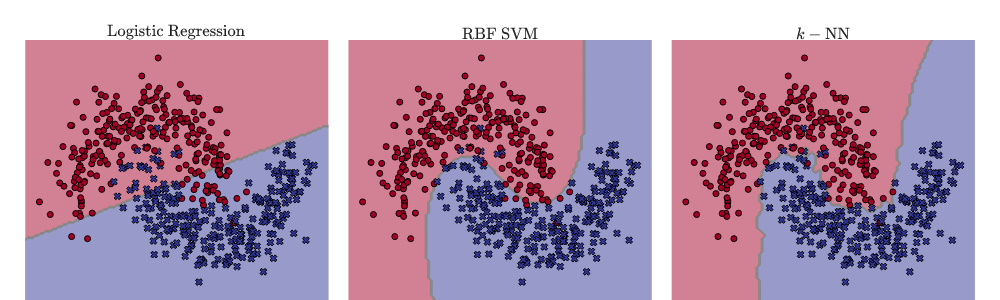
\includegraphics[width=.9\textwidth]{chapters/classification/figures/decision_boundary.png}
	\caption{\textbf{Decision Boundaries} of classifiers fitted over moons dataset. \GitChapterThreeExamples}
\end{figure}

\subsection{ROC Curve}\label{roc}
As we will encounter later in this chapter, in many classification scenarios we face the following question: Suppose we trained some classifier $h\in \Hc$ and derive classifications by the following rule: for some cutoff value $\alpha \in \left[0,1\right]$ $$\widehat{y}\coloneqq\begin{cases}
1 & h\left(\x\right)>\alpha\\
0 & h\left(\x\right)\leq\alpha
\end{cases}$$
How do we choose $\alpha$? There is an important \textbf{tradeoff} in the selection of $\alpha$. If we set $\alpha$ to be very high we are mainly going to predict $0$. By doing so we are \textbf{less} likely to have false-positives (which is the error we try to avoid at all cost), for which we are pleased. However, at the same time, we are \text{bf} more likely to gave false-negatives. So by setting $\alpha$ too high we might have low a FPR but "miss" (misclassify) most of the positive samples. On the other extreme, if we set $\alpha$ to be very low we are mainly going to predict $1$. So we will be \textbf{more} likely to have false-positives, but at the same time will be \textbf{less} likely to have false-negatives. So if we set $\alpha$ too low, we might have a high FPR but "catch" (correctly classify) most of the positive samples. Therefore, we see that changing $\alpha\in\left[0,1\right]$ governs some trade-off between the chances of making a Type-I error (false-positives) and correctly classifying positive samples.
\\~\\
This trade-off was first studied during World War II, when radar was invented. The designer of the radar had to choose when to put a green dot on the radar, indicating a target detected there. Sometime radar waves would bounce off back from clouds or birds, and the designer had to choose a \textbf{threshold} $\alpha$. If the radar pulse returning is stronger than $\alpha$, the radar screen would show a green dot. If weaker than $\alpha$, no dot. Now, if $\alpha$ is set too low (say $\alpha=0.1$), the screen would be full of a thousand green dots - since any bird or cloud (with, say, $h\left(\x=0.2\right)$) would be classified as \textbf{positive}, a target. So that the radar will be full of false positives, false targets, and will be useless. On the other hand, if $\alpha$ is set too high (say $\alpha=0.9$) then enemy airplanes  (with, say, $h\left(\x=0.8\right)$) will not appear on the screen, since they will be classified by mistake as birds, and the radar again would be useless. 

\begin{figure}[h!]
	\centering
	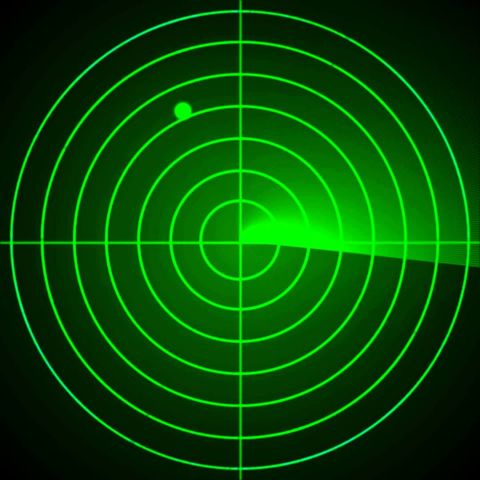
\includegraphics[width=1.7in]{chapters/classification/figures/radar.jpg}
	\caption{\todo{Change to caricature of planes dressed up as birds/clounds - and a confused radar}}
\end{figure}

The radar engineers developed a way to visualize this tradeoff, which is still used today in machine learning. After training some linear model (choosing some hypothesis $h\in\Hc$) we make a grid of values of $\alpha\in\left[0,1\right]$. For each value of $\alpha$ we create a classifier by thresholding  $h$ at $\alpha$, and calculate the number of  Type-I and Type-II errors the classifier makes over a test sample that was not used for training.  We plot a parametric curve of TPR (true positive rate) against FPR (false positive rate) when $\alpha$ is the parameter. This curve is called the \textbf{Receiver Operating Characteristic (ROC)} curve. It is continuous, increasing and goes from $(0,0)$ in the FPR-TPR plane (for $\alpha=0$ we classify everything as negative, so no false positives and not true positives) to $(1,1)$ (for $\alpha=1$ we classify everything as positive, so false positive rate is $1$ - we make every possible Type-I error - and also true positive rate is $1$ - we ``catch`` all the positive samples).

\begin{figure}[h!]
	\centering
	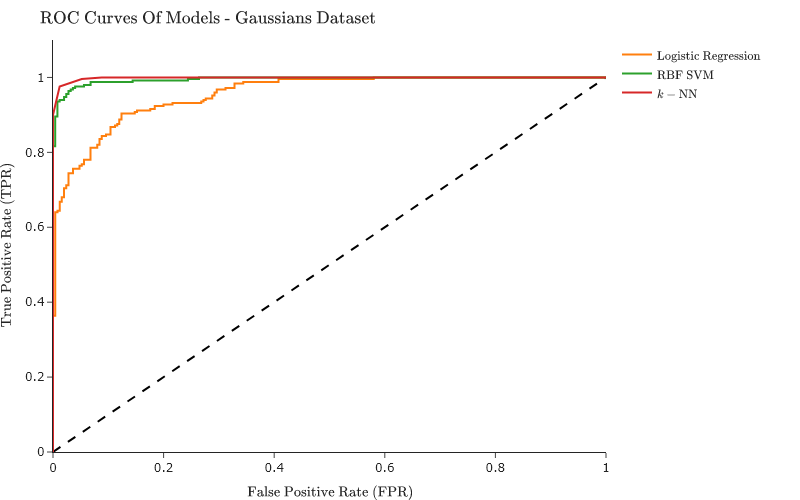
\includegraphics[width=.75\textwidth]{chapters/classification/figures/roc.png}
	\caption{\textbf{ROC Curve} of classifiers fitted over moons dataset. \GitChapterThreeExamples}
\end{figure}

Convince yourself that if the ROC curve is a linear line from $(0,0)$ to $(1,1)$, the classifier is just a random guess. If a classifier has an ROC curve that is closed to this linear line, it's a poor classifier. Now convince yourself that if the ROC curve rises sharply from $(0,0)$, for example makes a ``jump'' to $(FPR=0.1, TPR=0.9)$, it's a good classifier - we are able to correctly detect $0.9$ of the positive samples at the price of $0.1$ false positive rate. 
\\~\\
Plotting the ROC curve of a classifier has a few different uses:
\begin{itemize}
\item \textbf{Tuning $\alpha$:} It allows us to see the tradeoff, provided by the classifier, between Type-I errors and correct detection of positive samples, so we can choose the tuning of $\alpha$ we would like to work with for the actual prediction.
\item \textbf{AUC - Area Under Curve:} A performance measure for the tradeoff itself. This performance measure evaluates the prediction rule $h$ we chose without having to decide on $\alpha$ - it measures the quality of the \textbf{tradeoff} provided by $h$, a tradeoff from which we must choose a specific point in order to actually classify new samples. AUC is simply the \textbf{definite integral} of the ROC curve on the segment $[0,1]$ - the area under the AUC curve. As mentioned above, AUC around $1/2$ means that $h$ is poor - more specifically, that the \textbf{tradeoff} provided by $h$ is poor. AUC is bounded from above by $1$, so an AUC close to $1$ means $h$ offers an excellent trade-off, and in this case we expect to be able to find a cutoff $\alpha$ that gives a classifier with very few false-positives and very high detection rate (true positive rate).
\item \textbf{Comparing candidate rules:} Suppose we have a couple of candidate rules $h_1,h_2$ (or more). For example, maybe we trained some classifier on the same training sample with different features, or maybe we trained two different types of classifiers over the same data, and we are wondering which one to use. Now we have a problem - we can't turn $h_i$ into an actual classification rule without choosing a cutoff $\alpha_i$, but would like to compare $h_1$ to $h_2$ without committing to a cutoff - to compare the tradeoff offered by $h_1$ to that offered by $h_2$. It is very useful here to plot the two ROC curves of $h_1$ and $h_2$ on a single axis - and visually compare the tradeoffs they offer. 
\end{itemize}



\section{Half-Space Classifier}
Similar to linear regression, one of the simplest families of classifiers is that of linear classifiers. In these, we are interested in separating a given dataset into two classes using a linear separator function, as seen in \autoref{lin_sep1}.

\begin{figure}[h!] %TODO - caption should not be centered
	\centering
	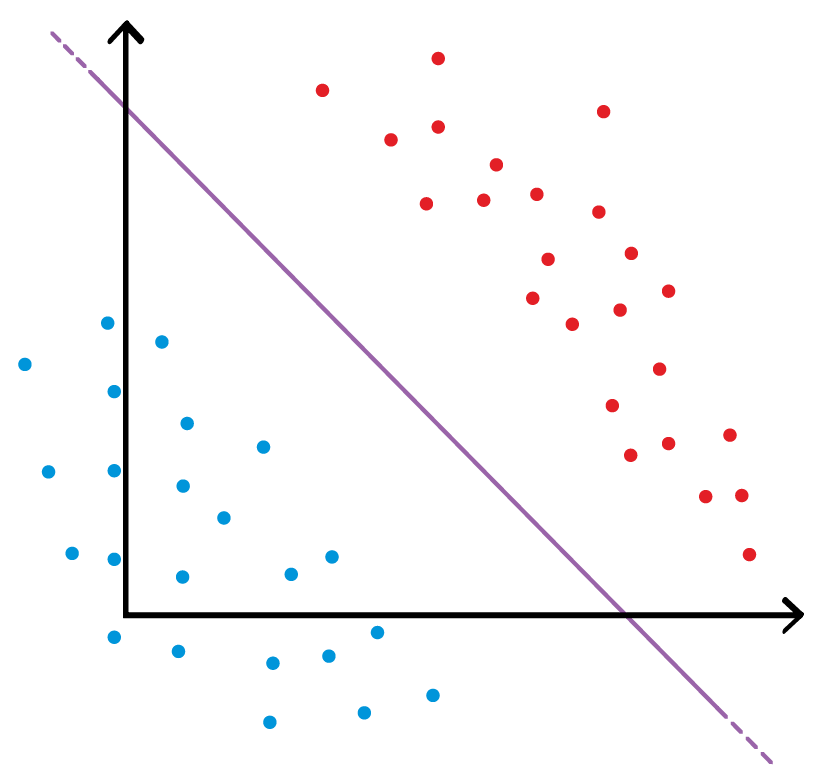
\includegraphics[width=0.4\textwidth]{chapters/classification/figures/3_1.png}
	\caption{Half-space Classification Illustration:} For a domain-set $\Xc\in\R^2$ the two classes, coded as red and blue colors, are linearly separable \label{lin_sep1}
\end{figure}

As we have seen in \autoref{eqn:lin_reg_h}, the family of linear functions can be described as: $$ L_d \coloneqq \left\{\x\mapsto \x^\top \w + b | \w\in\R^d,b\in\R\right\} $$
where the linearity refers to the functions being linear in the parameters $\w$. Next, consider the following definitions:

\begin{definition}\label{def:hyperplane}
Let $\w\in\R^d$ and $b\in\R$. The hyperplane defined by $\left(\w,b\right)$ is the set $$\left\{\x|\inprod{\w}{\x}=b,\,\x\in\R^d\right\}$$
\end{definition}
\begin{definition}\label{def:halfspace}
Let $\left(\w,b\right)$ be an hyperplane, so the half-space of $\left(\w,b\right)$ is defined as the set $$\left\{\x|\inprod{\w}{\x}\geq b, \x\in\R^d\right\}$$or equivalently as $\left\{\x|sign\left(\inprod{\w}{\x} - b\right)\geq 0,\x\in\R^d\right\}$.
\end{definition}

~\\Notice that the family of linear functions $L_d$ is in-fact the family of hyperplanes. As such, we can look at the family of functions that is the composition of the $sign$ function and $L_d$, $sign\circ L_{d}$. This family defines the hypothesis class of the half-space classifiers. Denote $h_{\w,b}\left(\x\right) = \inprod{\w}{\x} + b$ then:
\begin{equation}
\Hc_{half} \coloneqq \left\{h_{\w,b}\left(\x\right)=sign\left(\inprod{\x}{\w} + b\right)|\w\in\R^d,b\in\R\right\} = \left\{\x\mapsto sign\left(\inprod{\x}{\w}+b\right)\right\}
\label{eqn:h_half}
\end{equation}

~\\So why are functions in the form seen in \ref{eqn:h_half} are half-space classifiers? Let us assume at first that $b=0$. We can express the domain set as a disjoint union of the following:
$$ \R^d=\left\{\x\in\R^d | \w^\top \w>0\right\} \biguplus \left\{\x\in\R^d | \w^\top \w=0\right\} \biguplus \left\{\x\in\R^d | \w^\top \w<0\right\} $$
These sets correspond to the open half spaces on either side of the hyperplane $\w^\perp=\left\{\x\in\R^d|\w^\top \w=0\right\}$ and points on the hyper-plane itself. As such. each vector $\w\in\R^d$ defines a hyper-plane $\w^\perp$ that divides $\R^d$ into two half-spaces.

\begin{figure}[h!]
	\centering
	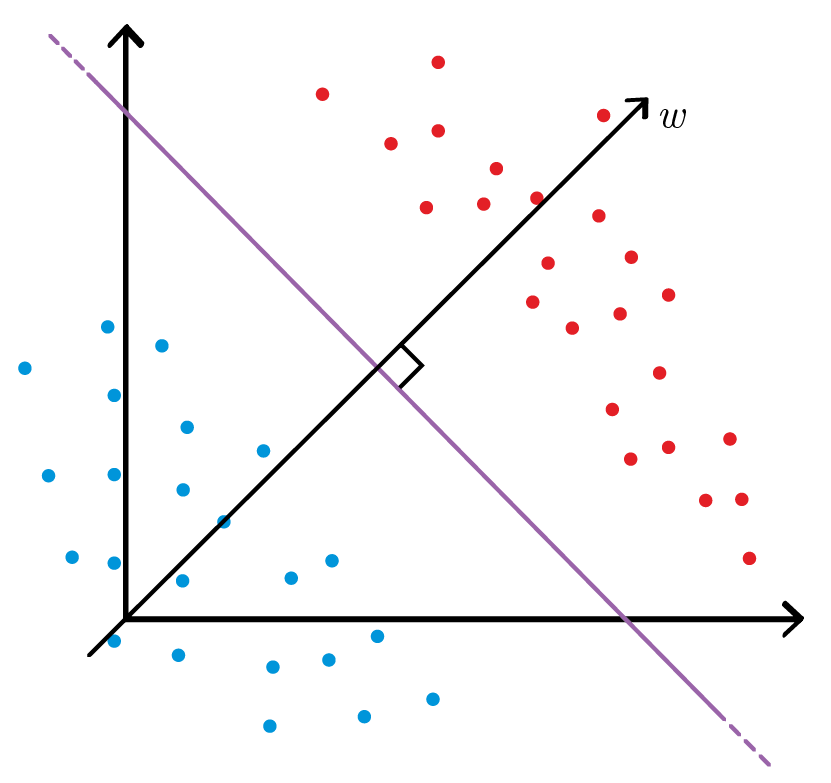
\includegraphics[width=0.4\textwidth]{chapters/classification/figures/3_2.png}
	\caption{Corresponding Hyperplane to $\w^\perp$}
\end{figure}

The case where $b=0$ is called the \textbf{homogeneous} case, as the hyperplane $\w^\perp$ is a linear subspace going through the origin. When $b\neq 0$ the hyperplane does not go through the origin and is called the non-homogeneous case. Recall that we have seen how we could transition from the non-homogeneous to the homogeneous case in the linear regression chapter.
\\~\\
Given a sample \trainset, we would like to find an hypothesis $h_{\w,b}\in\Hc_{half}$ such that all data points in $S$ that are labeled $1$ are on the one side of the hyper-plane and all those labeled $-1$ are on the other side. To find such an hypothesis we must first make the assumption that the dataset is \textbf{linearly separable}. That is, there exists a hyper-plane such that samples of opposing labels are on opposite sides. Mathematically, we assume that $$ \exists \w\in\R^d,b\in\R\quad s.t\quad \forall i\in\left[m\right] \quad y_i\cdot sign \left(\inprod{\x}{\w} + b\right)=1$$

or equivalently since the inner product will be negative for all samples with $y_i<0$ and positive for all samples with $y_i>0$:
$$ \exists \w\in\R^d,b\in\R\quad s.t\quad \forall i\in\left[m\right] \quad y_i\cdot \left(\inprod{\x}{\w} + b\right)>0$$

Note, that assuming that a given training set is linearly separable is a \textbf{realizability assumption}. Namely, the labels are generated by a function in our hypothesis class $\Hc_{half}$.

\subsection{Learning Linearly Separable Data Via ERM}
To train a model over the defined hypothesis class of homogenous half-spaces ($\w\in\R^d, b=0$) observe the following: For any hypothesis $h_\w\in \Hc_{half}$, the misclassified training samples are exactly those where $y_i\cdot sign\left(\inprod{\x}{\w}\right)=-1$ or equivalently $y_i\inprod{\x}{\w}<0$. So defining the loss of a given hypothesis over $S$ is: $$ L_S\left(h_\w\right)\coloneqq\sum^m_{i=1}\mathbbm{1}\left[y_i\inprod{\x}{\w}<0\right] $$

Since we assumed that $S$ is linearly separable, we would like to find $h_\w\in\Hc_{half}$ that perfectly separates the training set. Such an hypothesis will be one that achieves $L_S\left(h_\w\right)=0$. In other words, we are applying the ERM principle and seeking for any separating hyperplane $\w^\perp$, corresponding to an hypothesis $h_\w$ that minimizes the empirical risk $L_S\left(h_\w\right)$.

\subsection{Computational Implementation}
Once we realize what learning principle we want to apply, we need to find a compulationally efficient algorithm to find the desired hypothesis. As we are applying the ERM principle we would like to efficiently compute $$ \underset{\w\in\R^d}{argmin}\,L_S\left(h_\w\right) $$

As we are assuming the given sample is linearly separable (realazibility), there exists a vector $\w_0\in\R^d$ such that $ y_i\cdot\inprod{\x}{\w_0}>0\quad i=1,\ldots,m $. This implies that there also exists a (different) vector $\w_1\in\R^d$ such that $ y_i\cdot\inprod{\x}{\w_01}\geq 1 \quad i=1,\ldots,m $ as we can simply normalize $\w_0$ by the smallest product: $$ \w_1 \coloneqq \frac{1}{min_i\left\{y_i\cdot \inprod{\x}{\w_0}\right\}}\cdot \w_0 $$

Thus, it is enough to search for a vector $\w$ that satisfies $\forall\, i\in\left[m\right]\quad y_i\cdot sign\left(\inprod{\x}{\w}\right)\geq 1$. This is a problem of finding a vector that satisfies $m$ linear constraints, and can be solved using generic linear programming solvers. We are interested in solving:
\begin{equation}
\begin{array}{ccc}
minimize & L_S\left(h_{\w}\right) & \\
subject \, to & y_i\inprod{\x_i}{\w}\geq 1 & i=1,\ldots,m\\
\end{array}
\label{eqn:half_space_opt}
\end{equation}
which, as stated above for any ERM solution $L_S\left(h_\w\right)=0$. Therefore, as this optimization problem has a trivial objective, it is a \textbf{feasibility} problem - we are looking for any vector which satisfies the constraints.

\todo{ Proper writing+ deriving that this a a LP}

\subsection{The Perceptron Algorithm}
Another way for solving ERM for half-spaces is by using the Perceptron algorithm, suggested by Frank Rosenblatt in 1958. This is an iterative algorithm that constructs a series of vectors $\w^{\left(0\right)},\w^{\left(1\right)},\ldots$, each derived from the previous. At each iteration $t$ we search for a sample $i$ which is misclassified by $w^{\left(t\right)}$. Then, we update $\w^{\left(t\right)}$ by moving it in the direction of thhe misclassified sample $\w^{\left(t+1\right)}=\w^{\left(t\right)} + y_i\x_i$. 
\todo{ Add animation of perceptron}
\begin{algorithm}
	\caption{Batch-Perceptron}\label{batch_perceptron}
	\begin{algorithmic}
		\Procedure{Perceptron}{$\trainset$}
		\State $\w^{\left(0\right)} \gets 0$ \Comment{Initialize parameters}
		\For{$t=1,2,\ldots$}
		\If{$\exists \, i\,\, s.t. \,\,\, y_i\inprod{\w^{\left(t\right)}}{\x_i}\leq 0$}
		\State $\w^{\left(t+1\right)}=\w^{\left(t\right)}+y_i\x_i$
		\Else
		\State \textbf{return} $\w^{\left(t\right)}$
		\EndIf
		\EndFor
		\EndProcedure
	\end{algorithmic}
\end{algorithm}


\todo{ Add convergence + correctness theorem}

\begin{remark}
The Perceptron algorithm is in fact a simple case of the more general algorithm of Subgradient Descent covered in \autoref{chap:conv_opt}. Furthermore, we can modify the algorithm is such a way that rather than requiring an entire dataset $S$, it will each time get a single sample and update based on that one sample. We will encounter this variation in Online Learning \autoref{chap:online}.
\end{remark}


\section{Support Vector Machines}
When using the half-space classifier seen above we encounter two problems:
\begin{itemize}
	\item When we are searching for a separating half-space the solution is not unique. That is, there could be more than a single vector satisfying the constraints of \ref{eqn:half_space_opt} and achieving the minimal empirical loss (of zero when assuming realizibility or any other positive number if not). As such we are faced with the problem of which one to choose. \autoref{fig:multiple_hyperplanes} illustrates the existance of multiple separating hyper-planes. \\
	\item A more severe problem rises when we chose to work with the ERM learning principle for selecting the hypothesis, but the data is not linearly separable (non-realizible case). In this case the optimization problem described in \ref{eqn:half_space_opt} is computationally hard.
\end{itemize}


\begin{figure}[h!]
	\centering
	\begin{subfigure}[t]{0.35\textwidth}
		\centering
		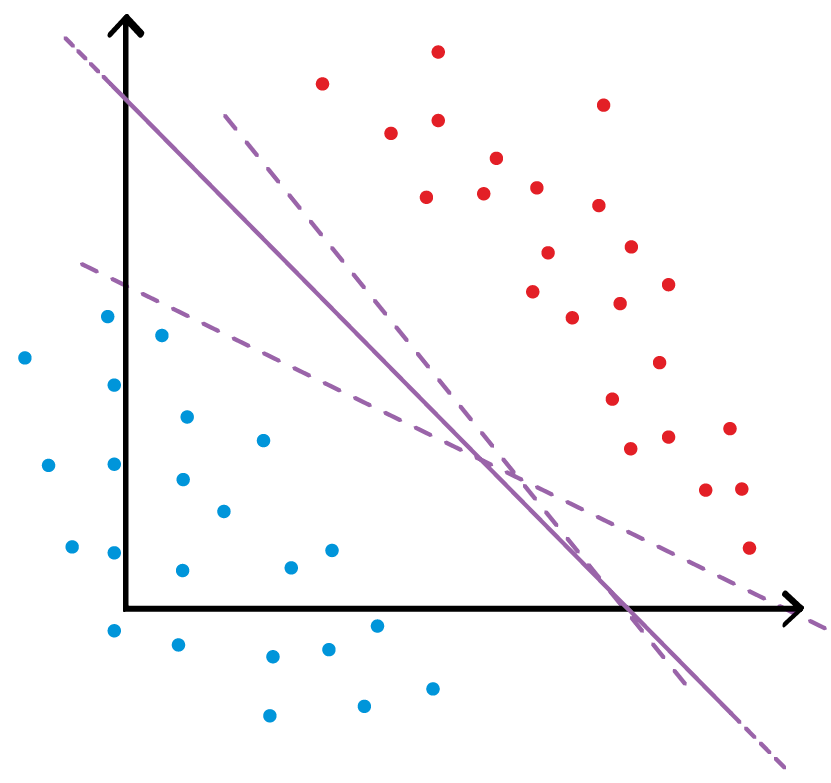
\includegraphics[width=\linewidth]{chapters/classification/figures/3_3.png}
		\caption{Algorithm selected hyper-plane (solid line) and additional optional separating hyperplanes (dashed lines)}
	\end{subfigure}
	\hspace{10mm}
	\begin{subfigure}[t]{0.35\textwidth}
		\centering
		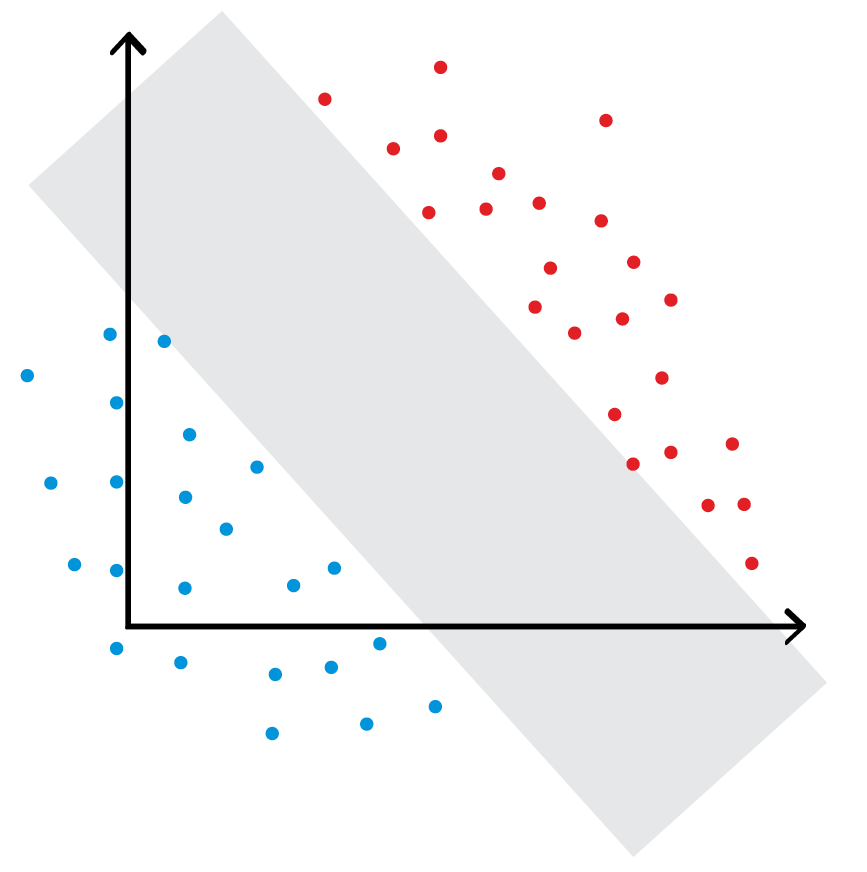
\includegraphics[width=\linewidth]{chapters/classification/figures/3_4.png}
		\caption{All hyper-planes linearly separating the data}
	\end{subfigure}
	\caption{Illustration of the existance of multiple separating hyper-planes}
	\label{fig:multiple_hyperplanes}
\end{figure}



~\\Returning to the same hypothesis class of non-homogeneous separating half-spaces $\Hc_{half}$ (\ref{eqn:h_half}), let us \textbf{not} assume the data is linearly separable. We would like to describe a different learning principle that will be able to cope with both problems above: finds a unique hypoerplane and that can be implemented computationally efficiently even when data is not linearly separable (i.e with polynomial running time given the input).

\subsection{Maximum Margin Learning Principle}

\begin{definition}
Let $\left(\w,b\right)\in \R^d\times\R$ be a hyperplane and $u\in\R^d$. Define the distance between $\left(\w,b\right)$ and $u$ by: $$ d\left(\left(\w,b\right),u\right)\coloneqq \underset{v:\inprod{v}{w}+b=0}{min}\left|\left|u-v\right|\right| $$ (namely, the Euclidean distance between $u$ and the closest point on the hyperplane)
\end{definition}

\begin{definition}[Margin]\label{def:margin}
Let $\left(\w,b\right)\in \R^d\times\R$ be a hyperplane and $S=u_1,\ldots,u_m\in\R^d$ a set of points. The \textbf{margin} of $\left(\w,b\right)$ and $S$ is the smallest distance between the hyperplane and any point: $$ M\left(\left(\w,b\right),S\right) \coloneqq \underset{i\in\left[m\right]}{min}\,\, d\left(\left(\w,b\right),u_i\right) $$
\end{definition}

So, the new learning principle is: choose $h_{\w,b}\in\Hc_{SVM}$ that has the \textbf{largest margin} with respect to our training data $S$. In \autoref{fig:margin} we are able to see that the margins of both hyper-planes. Based on that, we would prefer selecting the hyper-plane that is in the center of the grey area. The vectors closest to the hyperplane determine the margin. They are called \textbf{support vectors} and hence this learner's name.

\begin{figure}[h!]
	\centering
	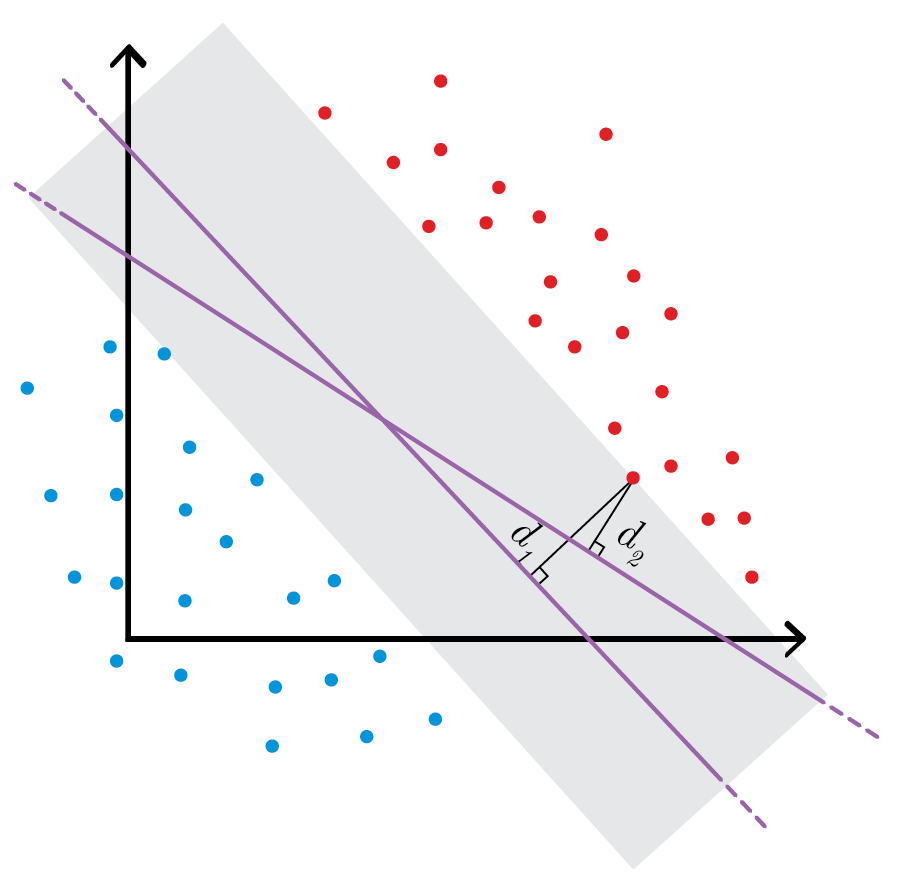
\includegraphics[width=0.4\textwidth]{chapters/classification/figures/3_5.png}
	\caption{Margin of specified hyper-planes}
	\label{fig:margin}
\end{figure}



\subsection{Hard-SVM}
Let's start with the \textbf{realizable case}. To implement our learning principle of maximal margin, we need to search, among all the hyperplane separating $S$, for the hyperplane with maximum margin. Namely, the hypothesis $h_{\w,b} \in \Hc_{SVM}$ our learner will choose is the solution to the following optimization problem:
\begin{equation}
\begin{array}{ccc}
maximize & M( (\w,b) , S) & \\
subject \, to & y_i \cdot \left( \inprod{\x_i}{\w}+b \right) \geq 1 & i=1,\ldots,m\\
\end{array}
\label{eqn:hard_svm_opt}
\end{equation}
The optimization variables are $\w\in\R^d,b\in\R$. Comparing with the linear program of half-spaces (\ref{eqn:half_space_opt}) we see that the constraints are kept, which ensure the hyperplane chosen separates the training sample, but instead of a trivial objective, we seek to minimize the margin (We don't worry about ``maximize`` instead of ``minimize`` as we can just multiply the objective by $-1$). 

\subsubsection{Convex Optimization}
The Hard-SVM optimization problem \ref{eqn:hard_svm_opt} (and many other problems we will encounter throughout the course) is part of a wide family of \textbf{convex optimization problems}.

\begin{definition}[Optimization Problem]
An optimization problem over $\R^d$ has the general form:
\begin{equation*}
\begin{array}{ccc}
minimize & f_0\left(\x\right) & \\
subject \, to & f_i\left(\x\right)\leq b_i & i=1,\ldots,n\\
\end{array}
\end{equation*}
where $\x$ is the optimization variable, $f_0:\R^d\rightarrow\R$ is the objective function and $f_i:\R^d\rightarrow\R$ are the constraint functions. It is implicitly implied that the optimization problem happens over $dom\left(f_0\right)\subset\R^d$, the domain of $f_0$.
\end{definition}

\begin{definition}[Convex Set]
Let $S$ be a vector space over the field of $\R$. A subset of $S$, $C\subseteq S$ is convex if and only if $\forall \vv{v},\vv{u}\in C $ the line connecting $\vv{v}$ and $\vv{u}$ is included in $C$. Equivenantly it means that $\forall \alpha\in\left[0,1\right]$ it holds that the convex combination $\left(1-\alpha\right)\vv{v}+ \alpha\vv{u}$ is included in $C$.
\end{definition}

\begin{definition}[Convex Function]
A function $f:\R^d\rightarrow\R$ is a convex function of $dom\left(f\right)$ is a convext set in $\R^d$, namely: $$ \forall\alpha,\beta\in\R\,\,\forall\vv{v},\vv{u}\in dom\left(f\right)\quad f\left(\alpha\vv{v}+\beta\vv{u}\right) \leq \alpha f\left(\vv{v}\right) + \beta f\left(\vv{u}\right)$$
\end{definition}

Then, naturally, a convex optimization problem is an optimization problem as above in which $f_0,f_1,\ldots,f_n$ are all convex functions. When these functions are all linear, this is a linear programming problem (as for example in \ref{eqn:half_space_opt}).

\begin{definition}[Quadratic Program]
An optimization problem is called a Quadratic Program (QP) if it can be written in the following form:
$$
\begin{array}{ccc}
\underset{\w\in\R^n}{min} & \frac{1}{2}\w^\perp Q\w + \vv{a}^\perp\w & \\
such\,that & A\w \leq \vv{d} \\
\end{array}
$$
where $Q\in\R^{n\times n}, A\in\R^{m\times n},\vv{a}\in\R^n,\vv{d}\in\R^m$ are fixed vectors and matrices.
\end{definition}

In general, optimization problems are hard to solve computationally. We take special interest in \textbf{convex optimization} problems since there have a unique solution, and that solution can be found in  computationally tractable ways. A great deal is known about \textbf{convex optimization algorithms}, which are iterative numerical algorithms that converge to the solution of a convex optimization problem. There are general solvers, which will solve a convex problem in the general form above, and there are specialized solvers for specific types, or families, of convex optimization problems. A specialized solver is typically preferred, as it leverages some particular structure of the problem to solve it more efficiently, using less space, etc. One example for specialized solvers you've seen in Algorithms course are specialized solvers for linear programs.
\\~\\
Why is convex optimization interesting for machine learning? In supervised learning, we would like to choose a hypothesis $h\in\Hc$ from our selected hypothesis class, based on some learning principle (such as ERM). Many learning principles are formulated as optimization problems, namely, the $h$ our learning algorithm chooses is given as the minimizer of some quantity (such as empirical risk). So implementation of the learning algorithm needs to solve an optimization problem. 
\\~\\
Sometimes, our hypothesis class is equivalent to a Euclidean space (for example, in linear regression we saw that linear functions are determined by the weight vector and an intercept, so the hypothesis class of linear functions was equivalent to the Euclidean space $\R^{d+1}$, and we've just seen the same happens for the hypothesis class of half-space classifiers). When this happens, our learning principle reduces to solving an optimization problem, namely, the hypothesis we choose $h\in\Hc$ is found as a minimum over $\R^d$ or a subset of $\R^d$ of some objective function, usually a loss function. When this objective is convex, we can use convex optimization algorithms to implement our learning algorithm efficiently. In \autoref{chap:conv_opt} we dive deeper into theory and algorithms of convex optimization.


\subsubsection{Solving Hard-SVM}
So is the Hard-SVM a convex optimization problem? Recall, that by our optimization problem \ref{eqn:hard_svm_opt}, we are searching of a separating hyperplane that maximizes the margin from all points. As for any $c>0$ it holds that $\left(\w,b\right)=\left(c\w,cb\right)$ we can w.l.o.g constraint ourselfs to $\norm{\w}=1$. This way, each hyperlane has a unique vector $\w$ that corresponds to it.

\begin{definition}
	Let $\x\in\R^d$ and $B\subseteq\R^d$. The distance from $\x$ to $B$ is: $$\underset{\vv{v}\in B}{inf} \norm{\x-\vv{v}}^2 $$
\end{definition}

\begin{exercise}
	Let $\left(\w,b\right)\in \R^d\times\R$ be a hyperplane where $\left|\left|w\right|\right|=1$ and $\x\in\R^d$ then the distance between $\x$ and the hyperplane $\left(\w,b\right)$ is $\left|\inprod{\w}{\x}+b\right|$.
\end{exercise}
\begin{proof}
	To solve this we begin with defining some point in the hyperplane, calculate it's distance from $\x$ and then showing minimality. Let $\vv{v}\coloneqq\x-\left(\inprod{\w}{\x}+b\right)\cdot\w$. This point $\vv{v}$ is indeed in the hyperplane: 
	$$
	\begin{array}{ccl}
		\inprod{\w}{\vv{v}}+b & = & \inprod{\w}{\x-\left(\inprod{\w}{\x}+b\right)\cdot\w}+b\\
		& = & \inprod{\w}{\x}-\left(\inprod{\w}{\x}+b\right)\norm{\w}^{2}+b\\
		& = & \inprod{\w}{\x}-\inprod{\w}{\x}-b+b=0
	\end{array}
	$$
	with a distance from $x$  of: $$ \norm{\x-\vv{v}}=\left|\inprod{\w}{\x}+b\right|\cdot\norm{\w} = \left|\inprod{\w}{\x}+b\right|$$ 
	Lastly, let us conclude that such $\vv{v}$ is the closest point in the hyperplane to $\x$. Let $\vv{u}$ be some point in the hyperplane, then:
	$$
	\begin{array}{ccl}
		\norm{\x-\vv{u}}^{2} & = & \norm{\x-\vv{v}+\vv{v}-\vv{u}}^{2}\\
		& = & \norm{\x-\vv{v}}^{2}+\norm{\vv{v}-\vv{u}}^{2}+2\inprod{\x-\vv{v}}{\vv{v}-\vv{u}}\\
		& \geq & \norm{\x-\vv{v}}^{2}+2\inprod{\x-\vv{v}}{\vv{v}-\vv{u}}\\
		& = & \norm{\x-\vv{v}}^{2}+2\inprod{\left(\inprod{\w}{\x}+b\right)\w}{\vv{v}-\vv{u}}\\
		& = & \norm{\x-\vv{v}}^{2}+2\left(\inprod{\w}{\x}+b\right)\inprod{\w}{\vv{v}-\vv{u}}\\
		& = & \norm{\x-\vv{v}}^{2}+2\left(\inprod{\w}{\x}+b\right)\left(\inprod{\w}{\vv{v}}-\inprod{\w}{\vv{u}}\right)\\
		& = & \norm{\x-\vv{v}}^{2}
	\end{array}
	$$
\end{proof}


So, as the margin \ref{def:margin} between a given hyperplane $\left(\w,b\right)$ and a set of points $S$ is the minimal distance between the hyperplane and any point in the set, we derive that our optimization problem is infact of the form:
\begin{equation}
	\begin{array}{ccc}
		\underset{\norm{\w}=1,b}{argmax} & \underset{i\in\left[m\right]}{min}\,\left|\inprod{\w}{\x_i}+b\right| & \\
		subject \, to & y_i \cdot \left( \inprod{\x_i}{\w}+b \right) \geq 1 & i=1,\ldots,m\\
	\end{array}
	\label{eqn:hard_svm_opt2}
\end{equation}

While the constraints enforce $\w$ to define a separating hyperplane, the objective will make us choose a separating hyperplane with the maximal margin. To solve this problem numerically, we will need to perform a slight manipulation and write it in a different form.

\begin{claim}
	Let $\left(\vv{v}^*,c^*\right)$ be an optimal solution of:
	\begin{equation}
		\begin{array}{ccc}
			\underset{\left(\w,b\right)}{argmin} & \norm{\w}^2 & \\
			subject \, to & y_i \cdot \left( \inprod{\x_i}{\w}+b \right) \geq 1 & i=1,\ldots,m\\
		\end{array}
		\label{eqn:hard_svm_opt3}
	\end{equation}
	Then, $\w^*\coloneqq\gamma\vv{v}^*,b^*\coloneqq\gamma c^*$ for $\gamma=\norm{\vv{v}^*}^{-1}$ is an optimal solution for \ref{eqn:hard_svm_opt2}.
\end{claim}
\begin{proof}
	Let us begin with simplifying Equation \ref{eqn:hard_svm_opt2}. Consider a \textit{feasible} solution $\w$ to the problem (that is, statisfies all constraints). It holds that $\left|\inprod{\w}{\x_i}+b\right|=y_i\left(\inprod{\w}{\x_i}+b\right)$. Hence, we can rewrite Equation \ref{eqn:hard_svm_opt2} as:
	$$
	\begin{array}{ccc}
		\underset{\norm{\w}=1,b}{argmax} & \underset{i\in\left[m\right]}{min}\,y_i\left(\inprod{\w}{\x_i}+b\right) & \\
		subject \, to & y_i \cdot \left( \inprod{\x_i}{\w}+b \right) \geq 1 & i=1,\ldots,m\\
	\end{array}
	\label{eqn:hard_svm_opt2}
	$$
\end{proof}
Now, it is clear that the constraints are redundant. If $\w$ is infeasible then $min_i\,y_i\left(\inprod{\w}{\x_i}+b\right)< 0$, achieving a lower objective than any feasible solution. Therefore, we can re-write the problem as:
$$ \underset{\norm{\w}=1,b}{argmax} \quad \underset{i\in\left[m\right]}{min}\,y_i\left(\inprod{\w}{\x_i}+b\right)\quad\left(\mathbf{*}\right) $$
Next, let us examine Equation \ref{eqn:hard_svm_opt3}. Notice that an optimal solution $\vv{v}^*,c^*$ will always satisfy: $$\underset{i\in\left[m\right]}{min}\,y_i\left(\inprod{\vv{v}^*}{\x_i}+c^*\right)=1$$
Otherwise, we can divide $\vv{v}^*$ by a positive number and get a feasible solution with a lower objective. As scalar multiplication does not change the hyperplane denote $\gamma=\norm{\vv{v}^*}^{-1}$ and let $\w^*\coloneqq\gamma\vv{v}^*, b^*\coloneqq\gamma c^*$. Since $\left(\vv{v}^*,c^*\right)$ is a is the optimal solution of \ref{eqn:hard_svm_opt3} it must satisfy all constraints and is therefore a feasible solution for  $\left(\mathbf{*}\right)$ with an objective: $$\underset{i}{min}\, y_i\left(\inprod{\w^*}{\x_i}+b^*\right) = \underset{i}{min}\, y_i\left(\inprod{\gamma \vv{v}^*}{\x_i}+\gamma c^*\right) = \gamma$$

Assume towards contradiction that there is a solution $\left(\w_2,b_2\right)\neq \left(\w^*,b^*\right)$ achieving a higher objective: $$\underset{i}{min}\, y_i\left(\inprod{\gamma \w_2^*}{\x_i}+\gamma b_2^*\right) = \delta > \gamma$$

But then $\left(\w_2/\delta, b_2/\delta\right)$ is a feasible solution for \ref{eqn:hard_svm_opt3} which $\norm{\w_2/\delta}=\delta^{-1} < \gamma^{-1}$ contradicting optimality of $\left(\vv{v}^*,c^*\right)$.
\\~\\
This means in fact that maximizing the margin is equivalent to minimizing the size of the hyperplane. The optimization problem written in \ref{eqn:hard_svm_opt3} is a quadratic program for which there exist efficient solves. By using them to solve problem \ref{eqn:hard_svm_opt3} we can obtain an optimal solution for the Hard-SVM optimization problem.

\begin{remark}
	But so how is it that minimizing $\norm{\w}^2$ is equivalent to maximizing the margin? Let us denote the width of the total margin (i.e. the sum of margin from both sides) by $l$, and let $x_{+}$ and $x_{-}$ be the positive- and negative support vectors . To calculate the value of $l$ we will project the vector $x_{+} - x_{-}$ onto the normalized normal $\w$: 
	$$\begin{array}{ccl}
		l& = & \inprod{x_{+} - x_{-}}{\frac{\w}{\norm{\w}}}\\
		& = & \left(\inprod{x_{+}}{\w}-\inprod{x_{-}}{\w}\right)\norm{\w}\\
		& = & \left(1-b-\left(1-b\right)\right)/\norm{\w}\\
		& = & 2/\norm{\w}
	\end{array}$$
	where support vectors satisfy $y_i\left(\inprod{\w}{\x_i}+b\right)$ and that for positive samples $y_i=1$ and negative samples $y_i=-1$. This shows how minimizing $\norm{\w}$ maximizes $l$.
\end{remark}


\subsection{Soft-SVM}
The basic assumption of Hard-SVM is that the training sample is linearly separable. If that is not the case then the optimization problem has no solutions as for any candidate $\left(\w,b\right)$ at least one of the constraints $y_i\cdot\left(\inprod{\w}{\x_i}+b\right)\geq 1$ cannot be satisfied.
\\~\\
But what if the training sample is almost linearly separable? That is, what if most of the samples are linearly separable with only a few violating the constraints by ``not too much``? Recall that if $y_i\cdot\left(\inprod{\w}{\x_i}+b\right)<0$ then sample $\x_i$ is on the ``wrong side`` of the hyperplane. This means that: $$\exists \,\xi_i> 0\quad s.t.\quad y_i\cdot\left(\inprod{\w}{\x_i}+b\right) \geq 1-\xi_i $$ Therefore, sample $\x_i$ is on the "wrong" side of the \textbf{margin} by an amount proportional to $\xi_i$ (\autoref{fig:soft_svm}). To allow training samples to violate the constraints ``a little``, we modify the optimization problem to:

\begin{equation}
	\begin{array}{clc}
		minimize & \norm{\w}^2 & \\
		subject \, to & \begin{cases}
			y_i \cdot \left( \inprod{\x_i}{\w}+b \right) \geq 1-\xi_i & i=1,\ldots,m\\
			\xi_i \geq 0\quad \land\quad \frac{1}{m}\sum_{i=1}^m \xi_i \leq C & \\
		\end{cases}
	\end{array}
	\label{eqn:sofv_svm_opt}
\end{equation}
where $C>0$ is a constant we specify. The variables $\xi_1,\ldots,\xi_m$ are new auxiliary variables we introduce (sometimes known as slack variables). Notice that the larger we choose $C$ to be, the more violations of margin we allow. On the one hand, we want to allow ``noisy`` samples to violate the margin, so the hyperplane will ignore them. On the other hand, if we allow too many violations, we lose touch with the training sample and its structure. This is exactly the bias-variance trade-off: the larger $C$, the more freedom the learner has to ``chase after the training sample``.

\begin{figure}[H]
	\centering
	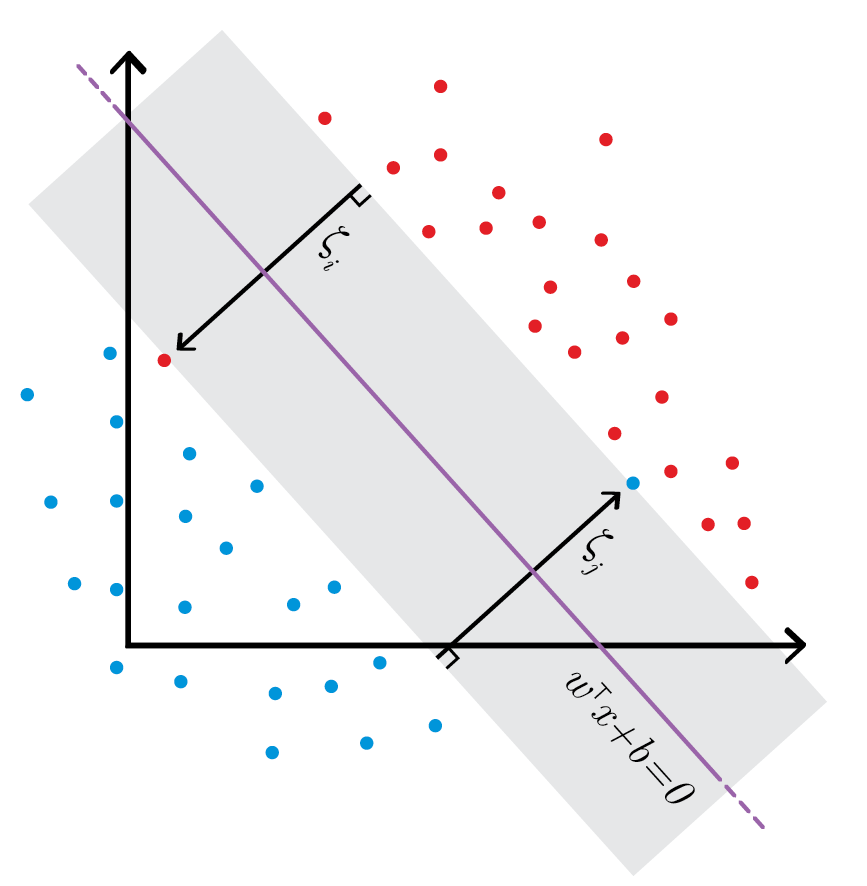
\includegraphics[width=0.3\textwidth]{chapters/classification/figures/3_6.png}
	\label{fig:soft_svm}
	\caption{Slack variables of data-points that are on the "wrong" side of the hyper-plane.}
\end{figure}
~\\
Instead of specifying $C$ directly, we often prefer working with a slightly different optimization problem, where instead of constraining the value of $\frac{1}{m}\sum\x_i$ we jointly minimize the norm of $\w$ (related to the margin) and the average of $\xi_i$ (corresponding margin violations).
\begin{equation}
	\begin{array}{cll}
		\underset{\w,\left\{\xi_i\right\}}{minimize} & \lambda\norm{\w}^2 + \frac{1}{m}\sum_{i=1}^m \xi_i& \\
		subject \, to & y_i \cdot \left( \inprod{\x_i}{\w}+b \right) \geq 1-\xi_i,\,\, \xi_i \geq0 & i=1,\ldots,m\\
	\end{array}
	\label{eqn:sofv_svm_opt}
\end{equation}

To simplify the above optimization problem let use define the \textbf{hinge} loss function:
\begin{equation}
	\ell^{hinge}\left(a\right)=\max\left\{0,1-a\right\},\,\, a\in\R
\end{equation}

\begin{claim}
	Given a training set $\trainset$ and hyperplane $\left(\w,b\right)$, the Soft-SVM optimization problem (\ref{eqn:sofv_svm_opt}) is equivalent to $$ \underset{\w,b}{\min} \left(\lambda\norm{\w}^2+L_S^{hinge}\left(\left(\w,b\right)\right)\right) $$ where $L_S^{hinge}\left(\left(\w,b\right)\right)\coloneqq \frac{1}{m}\sum \ell^{hinge}\left(y_i\inprod{\x_i}{\w}\right)$
\end{claim}

\begin{proof}
	Given a specific hyperplane $\left(\w,b\right)$ consider the minimization over $\xi_1,\ldots,\xi_m$. Since we defined the auxiliary variables to be nonnegative, the optimal assignment of $\xi_i$ is $$ \xi_i \coloneqq \begin{cases}
		0 & y_i\left(\inprod{\x_i}{\w}+b\right)\\
		1-y_i\left(\inprod{\x_i}{\w}+b\right) & otherwise\\
	\end{cases} $$
	Thus $\xi_i=\ell^{hinge}\left(y_i\left(\inprod{\x_i}{\w}+b\right)\right)$
\end{proof}

The hyper-parameter $\lambda$ controls the trade-off between the two norm of $\w$ and the violations of margin. The larger $\lambda$, the less sensitive the solution will be to the term $\frac{1}{m}\sum_{i=1}^m \xi_i$, and will allow more violations. The smaller $\lambda$, the more sensitive and will allow less violations. If we choose to work with this optimization problem to choose $h$, the constant $\lambda$ also moves us along different members of a family of learners, each with a different bias-variance tradeoff. $\lambda$ is known as a \textbf{regularization parameter}. This topic is covered in \autoref{chap:regularization}.



\subsection{Kernel Methods}\label{kernel_method}

The three classifiers seen above (halfspace classifier, Hard-SVM and Soft-SVM) all use the halfspaces hypothesis class. Though these linear classifiers are fairly simple to implement, the hypothesis class of halfspaces is of limited power. Consider the case where $\Xc=\R$ with the sample seen in \autoref{halfspace_lim_power} (left). As the data in not linearly separable, all three learners will fail. Notice however, that if instead of using the original feature representation of the data, we embed the samples in a new feature space, such as mapping each sample $x\rightarrow\left(x,x^2\right)$, we get a linearly separable sample in $\R^2$ (right).
\begin{figure}[H]
	\centering
	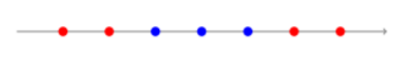
\includegraphics{chapters/classification/figures/linearly_inseparable.png}
	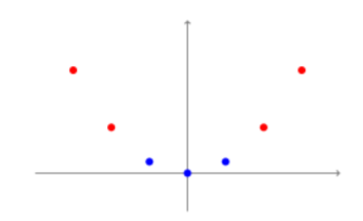
\includegraphics{chapters/classification/figures/linearly_separable.png}
	\caption{\textbf{Mapping to Feature Space}: Data originally linearly inseparable that is linearly separable in mapped feature space}\label{halfspace_lim_power}
\end{figure}

So, to enrich the expressiveness of an hypothesis class, we can consider embedding the data into another (potentially of higher dimension) feature space, over which we then learn some predictor. Schematically:
\begin{itemize}
	\item Given some domain set $\Xc\subseteq\R^d$ and a learning algorithm $\Ac$, select an embedding  $\psi:\Xc\rightarrow\Fc$ for some feature space $\Fc$. In many cases we will want $\Fc\subseteq \R^k$ for some $k \gg d$.
	\item Train $\Ac$ using the training set $\left\{\left(\psi\left(\x_i\right),y_i\right)\right\}^m_{i=1}$.
\end{itemize}~\\

This approach seems very attractive as the assumption that our data is linearly separable in \textit{some} feature space does not look very limiting. In order to apply this strategy, several challenges need to be addressed:
\begin{itemize}
	\item \textbf{Selection of $\psi$}: We need to find an appropriate mapping $\psi$ under which the data is linearly separable.
	\item \textbf{Computational complexity}:  Often, as $k\gg d$ (and sometimes even infinite) and as $\psi$ could be very complicated, computing $\psi\left(\x\right)$, is computationally expensive.
	\item \textbf{Sample complexity}: When transitioning to a potentially much higher feature space, the number of samples needed to learn a halfspace increases. \todo{Add reference to VCdim of halfspaces}
\end{itemize}
~\\
\begin{example}
	Suppose we are interested in separating between people that got a certain disease and people that don't, based on gene expression levels. We are given $\trainset$ where $\x_i$ is a vector in $\R^{20000}$ (the "gene space") where each coordinate $\x_i\left(j\right)$ denotes how much is gene $j$ expressed in individual $i$. $y_i\in\left\{\text{healthy},\text{sick}\right\}$ is the label. It is often the case that different genes are co-expressed, and modeling this co-expression might increase our expressive power and our ability to separate between the two groups. Let us create new additional features $\x_i\left(j\right)\x_i\left(k\right)$ that captures \textit{interaction} between the $j,k$ features. Using this mapping each sample gets the form: $$ \psi\left(\x\right) = \left(\x\left(1\right),\ldots,\x\left(20000\right),\x\left(1\right)\x\left(1\right),\ldots,\x\left(1\right)\x\left(20000\right),\ldots,\x\left(20000\right)\x\left(2000\right)\right)^\top $$ 
	Meaning that the feature space is of dimension $d+d^2/2=\mathcal{O}\left(d^2\right)$ where $d=20000$ the dimension of the original sample space. If we decide to use co-expression of geen trios then the feature space is of dimension $d+d^2/2 + d^3/3=\mathcal{O}\left(d^3\right)$. Depending on the problem it might make sense to also look at feature interactions of even higher orders, suppose interactions of $k$ features. If that is the case, our mapping function, maps us to a space of size $\mathcal{O}\left(d^k\right)$, which is exponential in the original sample space size.
\end{example}

\subsubsection{Kernel Functions}
As the mapping enables us to transition to a new feature space of very high dimension (could be exponential or even of infinite dimension), we are facting a computational challange in computing this transition. To address this problem we could use kernel based learning. In this approach, we decide to use a mapping function out of a (wide) specific family of mapping functions, called \textit{kernel functions}, that even though might map to a very high dimension, can still be computed efficiently.\\

\begin{definition}[PSD Kernel]
	A symmetric function $k:\Xc\times\Xc\rightarrow\R$ is called a Positive Semi-Definite kernel on $\Xc$ if $\forall \left\{x_1,\ldots,x_m\right\}\subseteq\Xc$ the associated kernel matrix (also known as Gram matrix) $K_{ij}=k\left(\x_i,\x_j\right)$ is PSD.
\end{definition}
\begin{corollary}
	Let $g:\Xc\times\Xc\rightarrow\R$ and $h:\R^d\rightarrow\R^k$ such that $g\left(x,y\right)=h\left(x\right)^\top h\left(y\right)$. Then $g$ is a PSD kernel function.
\end{corollary}
\begin{proof}
	Given a arbitrary set $\left\{\x_1,\ldots,\x_m\right\}\subseteq\Xc$ for arbitrary size $m\in\N$ denote $H$ the matrix where: $$ H=\left[\begin{array}{ccc}
		| & & |\\
		h\left(\x_1\right) & \cdots & h\left(\x_m\right)\\
		| & & |
	\end{array}\right] $$
	Consider the matrix $G=H^\top H$ so $G_{ij}=h\left(\x_i\right)^\top h\left(\x_j\right)=g\left(\x_i,\x_j\right)$. So $G$ is the Gram matrix of $g$ over the given set. This matrix is PSD as we were able to show it as the multiplication of $H^\top H$ \todo{add reference to PSD equiv. conditions}
\end{proof}

This corollary means that any kernel function can be written as an \textbf{inner product} of some transformation $h$ of the data. This transformation $h$ is the mapping function described above. So to check if a given function is a kernel function we could: $\left(1\right)$ show the associated Gram matrix is PSD or $\left(2\right)$ find the transformation $h$ that satisfies that $g\left(x,y\right)=h\left(x\right)^\top h\left(y\right)$~\\

\begin{exercise}
	Let $\Xc=\R^d$. Show that $k:\Xc\times\Xc\rightarrow \R$ that is defined by $k\left(x,y\right)=1,\,\,x,y\in\Xc$ is a valid kernel function. In addition, state a possible mapping function $h$ such that $g\left(x,y\right)=h\left(x\right)^\top \left(y\right)$.
\end{exercise}
\begin{proof}
	Let $\left\{\x_i\right\}^m_{i=1}\subseteq\Xc$. The Gram matrix of $k$ over this set is: $K_{ij}=k\left(\x_i,\x_j\right)=1$. As the eigenvalues of $K$ are $m,0\geq 0$ and $K$ is a symmetric matrix, we conclude that $K\in PSD$. Thus $k$ a valid kernel function.\\ As for the mapping function $h$, it must satisfy that $h\left(x\right)^\top h\left(y\right)=1$ for any $x,y$. So we could choose $h:\R^d\rightarrow\R^k$ that always returns some unit vector $v$. Then $h\left(x\right)^\top h\left(y\right) = v^\top v = \norm{v} = 1$. Notice that we haven't specificed $k$, the dimension of the embedded space, which could be of any size we desire.
\end{proof}


~\\One commonly used kernel function is the polynomial kernel.
\begin{claim}[Polynomial Kernels]
	Let $\Xc=\R^d$ and consider the $k$ degree polynomial mapping:$$\x\mapsto\left(1,\ldots,\x\left(i\right),\ldots,\x\left(i\right)\x\left(j\right),\ldots,\prod_{\underset{J\subset\left[d\right],\left|J\right|=k}{i\in J}}\x\left(i\right)\right)$$
	This is a valid kernel and can be computed by $$ k\left(\x,\x'\right)\coloneqq\left(1+\inprod{\x}{\x'}\right)^k $$
\end{claim}
\begin{proof}
	To show this is a valid kernel, we will find some mapping $\psi$ such that $K\left(\x,\x'\right)$ equals to $\psi\left(\x\right)^\top \psi\left(\x'\right)$. For simplicity let $x_0=1=x'_0$. Then: 
	$$
	\begin{array}{ccl}
		k\left(\x,\x'\right) & = &\left(1+\inprod{\x}{\x'}\right)^k\\
		& = & \left(\sum_{i=1}^d x_ix'_i\right)^k\\
		& = & \sum_{J\in\left\{0,\ldots,d\right\}^k}\prod_{i=1}^{k}x_{J_i}x'_{J_i}\\
		& = & \sum_{J\in\left\{0,\ldots,d\right\}^k}\prod_{i=1}^{k}x_{J_i}\prod_{i=1}^{k}x'_{J_i}\\
		& = & \sum_{J\in\left\{0,\ldots,d\right\}^k}\psi\left(\x\right)_J\psi\left(\x'\right)_J\\
		& = & \psi\left(\x\right)^\top \psi\left(\x'\right)
	\end{array}
	$$
	Where we define $\psi:\R^d\rightarrow\R^{\left(n+1\right)^k}$ such that each coordinate of $\psi\left(\x\right)$ corresponds to some $J\in\left\{0,\ldots,d\right\}^k$ and is equal to $\prod_{i=1}^k x_{J_i}$. Therefore we obtained that $k\left(\x,\x'\right) = \inprod{\psi\left(\x\right)}{\psi\left(\x'\right)}$
\end{proof}

~\\
\begin{example}
	Let $\x,\x'\in \Xc=\R^2$ with $x_0=1=x'_0$ and $k=2$ so:
	$$ \begin{array}{ccl}
		\left(1+\inprod{\x}{\x'}\right)^2 & = & \left(1+x_1x'_1 + x_2x'_2\right)^2\\
		& = & 1 + 2x_1x'_1 + 2x_2x'_2 + \left(x_1x'_1\right)^2 + \left(x_2x'_2\right)^2 + 2x_1x'_1x_2x'_2
	\end{array} $$
	By defining $\psi$ as $\psi\left(\x\right)=\left(1,1\cdot x_1, x_1 \cdot 1, 1\cdot x_2, x_2\cdot 1, x_1^2, x_2^2, x_1\cdot x_2, x_2 \cdot x_1\right)^\top$ we achieve that $K\left(\x,\x'\right)=\psi\left(\x\right)^\top \psi\left(\x'\right)$
\end{example}

~\\
\begin{claim}[Gaussian Kernels]
	The following is a valid kernel function: $$ k\left(\x,\x'\right)\coloneqq \exp\left(-\frac{1}{2\sigma^2}\norm{\x-\x'}^2\right),\quad\sigma^2\in\R_+ $$ with the mapping function $\psi$ defined such that: $$ \forall n\in\N \quad \psi\left(\x\right)_n \coloneqq \frac{1}{\sqrt{n!}}\exp\left(-x^2/2\sigma\right) x^n $$
\end{claim}
\begin{proof}
	Let us begin with showing that $k\left(\x,\x'\right) = \psi\left(\x\right)^\top \psi\left(\x'\right)$:
	$$
	\begin{array}{ccl}
		\psi\left(\x\right)^\top \psi\left(\x'\right) & = & \sum_{n=0}^\infty \left(\frac{1}{\sqrt{n!}}\exp\left(-x^2/2\sigma\right) x^n\right) \left(\frac{1}{\sqrt{n!}}\exp\left(-\left(\x'\right)^2/2\sigma\right) \left(\x'\right)^n\right)\\
		& = & \exp\left(-\frac{\x^2 +\left(\x'\right)^2}{2\sigma}\right)\sum_{n=0}^\infty \frac{\left(\x\x'\right)^n}{n!}\\
		& = & \exp\left(-\frac{1}{2\sigma^2}\norm{\x-\x'}^2\right)
	\end{array}
	$$
\end{proof}
Interestingly, the feature space mapped by $\psi$ is of infinite dimension.

~\\Since a function is a valid kernel function if it's associated Gram matrix is PSD we can derive several closure properties for kernel functions. Here are some of these properties.
\begin{claim}
	Let $k$ be some valid kernel function then the following are valid kernel functions:
	\begin{enumerate}
		\item $k\left(x,y\right)x^\top A y$, where $A\in PSD$.
		\item $c\cdot k_1\left(x,y\right)$ where $c>0$.
		\item $exp\left(k_1\left(x,y\right)\right)$
		\item $f\left(x\right)k_1 f\left(y\right)$
	\end{enumerate}
\end{claim}
\begin{exercise}
	Using the closure properties above, show that the Gaussian kernel is a valid kernel function.
\end{exercise}
\begin{proof}
	$$
	\begin{array}{ccl}
		k\left(\x,\x'\right) & = & \exp\left(-\norm{\x-\x'}^2/2\sigma^2\right) \\
		& = & \exp\left(-\norm{\x}^2/2\sigma^2\right) \cdot \exp\left(-\x^\top\x'/\sigma^2\right) \cdot \exp\left(-\norm{\x'}^2/2\sigma^2\right) \\
		& \overset{\left(*\right)}{=} & f\left(\x\right) \exp\left(-\x^\top\x'/\sigma^2\right) f\left(\x'\right) 
	\end{array}
	$$
	where we define $f\left(\x\right) = \exp\left(-\norm{\x}^2/2\sigma^2\right)$. Now notice that this is a valid kernel as: $\left(1\right)$ $\x^\top\x'$ is a valid kernel. $\left(2\right)$ scaling by $\frac{1}{\sigma^2}$ is a valid kenel. $\left(3\right)$ exponent of a valid kernel is a valid kernel. And finaly, $\left(4\right)$ multiplying by $f\left(\x\right), f\left(\x'\right)$ from left and right is a valid kernel.
\end{proof}

\begin{remark}
	The Gaussian kernel is a specific case of the wider Radial Basis Function (RBF) kernel $k\left(\x,\x'\right)\coloneqq \exp\left(-\beta \norm{\x-\x'}^2\right)$.
\end{remark}

~\\ Notice in both examples, the polynomial- and Gaussian kernels, the embedding is of much higher dimension but computing the value can be done efficiently without actually transitioning to the feature space. In the case of the $k$ degree polynomial kernel, the feature space is of dimension $\mathcal{O}\left(\left(d+1\right)^k\right)$. In the case of the Gaussian kernel the feature space is of an infinite dimension. However in both cases, computing the kernel function can be done in $\mathcal{O}\left(d\right)$.


\subsubsection{The Kernel Trick}
Now that we have introduced the notion of kernel functions, and seen that they encapsulate the mapping to some possibly-elaborate feature space, the next question is when and how can we apply it to different learning algorithms. Here we will use kernels in the context of the SVM algorithm and in \ref{kernel_pca} we use kernels in the context of the Kernel-PCA algorithm.
~\\
\todo{Add SVM using kernels - for that we need to state representer theorem}\\
\todo{Finish with: The algorithm must be written as inner products of the data}


\section{Logistic Regression}
\subsection{A Probabilistic Model For Noisy Labels}
Recall the statistical model for linear regression when assuming Gaussian errors (\ref{lin_reg_stat_model}), $\y=\X\w+\eps$ where $\eps\sim\Nc\left(0,\sigma^2I_d\right) $. Notice that as $\eps$ is a random variable, $\y$ too is a random variable distributing as a multi-variate Gaussian:
$$ \y\sim\Nc\left(\X\w,\sigma^2I_d\right) $$

Focusing on a pair $\left(\x_i,y_i\right)$, we can think of the above as the \textbf{conditional probability} of $y_i$ given $\x_i$: $$ p\left(y_i|\x_i,\w\right) =\Nc\left(y_i|\phi_{\w}\left(\x_i\right),\sigma^2\right)\quad \text{where}\quad \phi_{\w}\left(\x\right)=\w^\top\x$$
where we also condition on $\w$ to explicitly state the dependence on the model parameters. In other words, we assumed that each sample $\left(\x,y\right)$ is such that the \textbf{expected value} of the label $y$ is linear in $\x$. As we are dealing with a regression model and $y_i\in\R$, the support of the random variable $y_i|\x_i,\w$ is $\R$. 
\\~\\
Let us adapt the model above to fit for classification problems. We would like to assume that $y_i$ distributes \textbf{Bernoulli} with a probability $p\left(\x_i\right)$ that somehow relates with $\x_i$, and captures how likely is $y_i$ being $1$: $$ p\left(y_i|\x_i\right)=Ber\left(y_i|p\left(\x_i\right)\right) $$
How shall $p\left(\x_i\right)$ relate with $\x_i$? Unlike the linear regression model, we cannot assume a linear function $\phi_{\w}\left(\x\right)=\w^\top\x$ as $\phi_{\w}\in\R$ while $p\left(\x_i\right)$ is restricted to $\left[0,1\right]$. Instead, we would like to choose some \textbf{link} function $\phi_{\w}:\R\rightarrow\left[0,1\right]$ that is monotone increasing and maps $\left(-\infty,\infty\right)$ bijectively to $\left(0,1\right)$. Define the relation to be
\begin{equation}
	p\left(y_i|\x_i,\w\right) = Ber\left(y_i|\phi_{\w}\left(\x_i\right)\right), \quad \phi_{\w}\coloneqq sigm\left(\w^\top\x\right)
	\label{eqn:logistic_model}
\end{equation}
where $sigm$ is the \textbf{sigmoid} function, also known as the \textbf{logit} function: $$ sigm\left(\vv{a}\right)\coloneqq\frac{e^{\vv{a}}}{e^{\vv{a}} + 1} $$
This function is indeed monotone increasing and maps $\left(-\infty,\infty\right)$ bijectively to $\left(0,1\right)$.

\begin{figure}[h!]
	\centering
	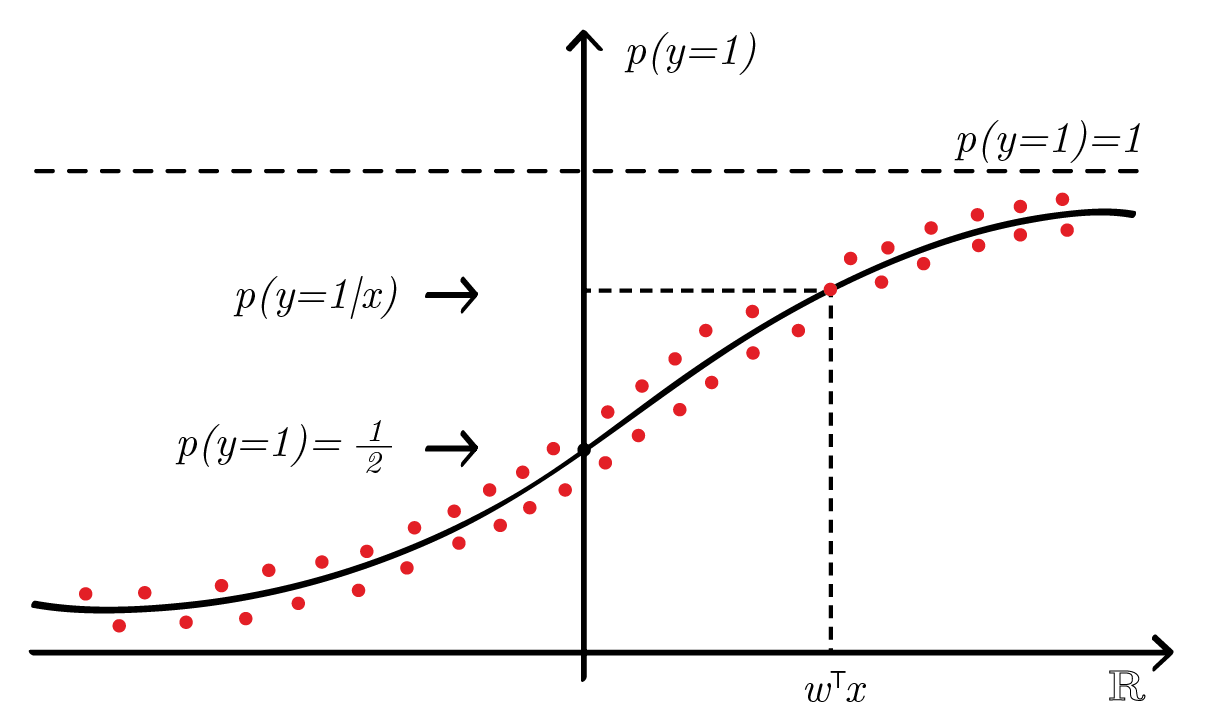
\includegraphics[width=0.5\textwidth]{chapters/classification/figures/3_7.png}
	\caption{\textbf{Illustration of fitted logit function} for values corresponding to $\w^\top x$.}
\end{figure}


\begin{itemize}
	\item As $\w^\top\x\rightarrow -\infty$ then $sigm\left(\w^\top\x\right)\rightarrow 0$. This means that it is ``very unlikely`` that the label is $1$:  $p\left(y_i=1|\x_i,\w\right)\rightarrow 0$. 
	\item As $\w^\top\x\rightarrow \infty$ then $sigm\left(\w^\top\x\right)\rightarrow 1$. This means that it is ``very likely`` that the label is $1$: $p\left(y_i=1|\x_i,\w\right)\rightarrow 1$. 
\end{itemize}


\begin{remark}
	In \ref{eqn:logistic_model} we modeled the logistic regression model for binary classification problems. Notice that the Bernoulli distribution can be seen as a private case of the Multinomial distribution $Multinomial\left(p_1,\ldots,p_K\right),\,\,\sum_pi=1, 0\leq p_i\leq 1$. We can expand the above logistic regression model to fit multi-classification problems by extending the sigmoidal function to what is known as the softmax function $\sigma\left(\vv{a}\right)=e^{\vv{a}_i}/\sum^K_{j=1}e^{\vv{a}_j}$
\end{remark}

\subsubsection{The Hypothesis Class}
So we would like to define the hypothesis class of logistic regression as: 
\begin{equation}
	\Hc_{logistic}\coloneqq\left\{h_{\w}\left(\x\right)=sigm\left(\w^\top\x\right)|\w\in\R^{d+1}\right\}
	\label{eqn:logisitc_hypothesis_class}
\end{equation}
However, notice that defining the hypotheses in such manner means that $h_{\w}:\R^{d+1}\rightarrow\left[0,1\right]$ and not $h_{\w}:\R^{d+1}\rightarrow\left\{0,1\right\}$ as required for classification problems. Since $\left\{0,1\right\}\subset\left[0,1\right]$, we can use the training sample to select a function in $\Hc_{logistic}$. This means we will be able to train a model, but how will we predict over new samples? Suppose our learner chose some $h_{\w}\in\Hc_{logistic}$. As we think about $h_{\w}\left(\x\right)$ as an estimate of the probability that the label corresponding to $\x$ is $1$, we can use it for classification. If $h_{\w}\left(\x\right)$ is low the label is likely to be $0$. If $h_{\w}\left(\x\right)$ is high, the label is likely to be $1$. Choosing some \textbf{cutoff} value $\alpha\in\left[0,1\right]$, our class prediction will be: $\widehat{y}\coloneqq \indc{h_{\w}\left(\x\right)>\alpha} $. To choose a fitting value for $\alpha$ we can calculate the Type-I and Type-II errors of the classifier and plot its ROC curve (\autoref{error_types} and \autoref{roc})


\subsubsection{Learning Via Maximum Likelihood}
Once we have defined the logistic regression model (\ref{eqn:logistic_model}) and hypothesis class (\ref{eqn:logisitc_hypothesis_class}), we would like to come up with a learner. To do so we will use the maximum likelihood principle. Recall, that by the maximum likelihood principle, we estimate the parameters (the desired hypothesis) as those that have the highest probability, given the data.
\\~\\
Let $\trainset$ be our sample of independent observations, assuming that $\y_i\sim Ber\left(\phi_{\w}\left(\x\right)\right)$ where $\phi$ is the logistic function. The likelihood of $\w\in\R^{d+1}$ is: 
$$
\begin{array}{ccl}
	\Lc\left(\w\right|\X,\y) & = & \Prob\left(y_1,\ldots,y_m|\X,\w\right) \,\, = \,\, \prod \Prob\left(y_i|\x_i,\w\right)\\
	& = & \underset{i:y_i=1}{\prod}\Prob\left(y_i|\x_i,\w\right)\cdot \underset{i:y_i=0}{\prod}\Prob\left(y_i|\x_i,\w\right)\\
	& = & \underset{i:y_i=1}{\prod} p_i\left(\w\right) \cdot \underset{i:y_i=0}{\prod} \left( 1-p_i\left(\w\right)\right)\\
	& = & \prod p_i\left(\w\right)^{y_i} \left(1-p_i\left(\w\right)\right)^{1-y_i}
\end{array}
$$
where $p_i\left(\w\right)=\phi_{\w}\left(\x_i\right)$. Since the log function is monotone increasing we can maximize the log-likelihood $\ell\left(\w\right)\coloneqq \log\Lc\left(\w\right)$ instead: $$
\begin{array}{ccl}
	\ell\left(\w|\X,\y\right) & = & \overset{m}{\underset{i=1}{\sum}}\left[y_i\log\left(p_i\left(\w\right)\right)+\left(1-y_i\right)\log\left(1-p_i\left(\w\right)\right)\right]\\
	& = & \overset{m}{\underset{i=1}{\sum}}\left[ y_i\log\left(\frac{e^{\w^\top \x_i}}{1+e^{\w^\top \x_i}}\right) + \left(1-y_i\right)\log\left(\frac{1}{1+e^{\w^\top\x_i}}\right) \right]\\
	& = & \overset{m}{\underset{i=1}{\sum}} \left[y_i\cdot \w^\top\x_i - \log\left(1+e^{\w^\top\x_i}\right)\right]
\end{array}
$$
And therefore, choosing the function $h\in\Hc_{logistic}$ by applying the maximum likelihood principle means that: 
\begin{equation}
	\widehat{\w}\coloneqq \underset{\w\in\R^{d+1}}{argmax} \overset{m}{\underset{i=1}{\sum}} \left[y_i\cdot \w^\top\x_i - \log\left(1+e^{\w^\top\x_i}\right)\right]
	\label{eqn:logistic_opt}
\end{equation}


\begin{remark}
	Instead of deriving the learner using the maximum likelihood principle, we could derive it using the ERM principle with the following loss function: $\ell\left(h_{\w}\right)\coloneqq \log\left(1+\exp\left(-y\inprod{\w}{\x}\right)\right)$. We would have reached the same optimization expression.
\end{remark}

\subsection{Computational Implementation}
Now that we have defined the hypothesis class and an optimization problem to find the desired hypothesis, the next step is finding an efficient algorithm to solve it. By working with the logistic function, the resulting log-likelihood expression is \textbf{concave} function of the optimization variable $\w$. This means, that instead of solving the maximization problem \ref{eqn:logistic_opt} we can solve the minimization of minus the log-likelihood, which is convex. As such, there are general algorithms for finding the minima of such functions.
\\~\\
While there is no closed form for the maximizer $\widehat{\w}$, as logistic regression is a very useful learner, there is a custom iterative algorithm that usually converges quickly to $\widehat{\w}$. This algorithm is based on \textbf{Newton-Raphson} iterations.


\subsection{Interpretability}
One important properly of the logistic regression learner is interpretability both in the sense of which features were important for the model and why was a certain prediction given. When working with $\Xc=\R^d$, we gather many feature, and might think that some of them are important for prediction while others less. Similar to linear regression, we are able to ask "which features were important" for the model by simply investigating the entries of the fitted coefficients vector $\w$. Feature corresponding to coefficients of values close to zero have a small impact on prediction and therefore these features are less important for the model. Features corresponding to coefficients of values far from zero have a large impact on prediction and are therefore important for the model.
\\~\\
Then, for a given sample $\x$, by looking at entries corresponding to important features we can understand why the model predicted $\widehat{y}$. If in entries of $\x$ corresponding important features there are large (positive or negative) values, they will have much influence the outcome. If these values are of same sign as of the coefficients then the expression $\w^\top\x$ will be larger, increasing the likelihood of the prediction being $1$. If these values are of opposite signs to the coefficients then the expression $\w^\top\x$ will become smaller, decreasing the likelihood of the prediction being $1$.



\section{Bayes Classifiers}
The logistic regression classifier seen above assumes a distribution on the labels $\Yc$ given the samples  
\todo{Matan - need to be written - Begin with defining $\Dc$ over $\Xc\times\Yc$}
\todo{Then add notions of posterior(likelihod), prior and joint distributions}

\subsection{Bayes Optimal Classifier}
\todo{From the above derive Bayes optimal}

\subsection{Naive Bayes}
\todo{From the above derive Naitve optimal}

\subsection{Linear Discriminant Analysis}
The Linear Discriminant Analysis (LDA) algorithm is yet another realization of the Bayes Optimal classifier. This time we assume that the points from each label have a different Gaussian distribution. Explicitly, we assume the following generative model: 
\begin{enumerate}
	\item Each sample selects a label $y_i=Ber\left(\pi\right),\,\,\pi\in\left[0,1\right]$.
	\item Then, the sample itself is drawn from the conditional probability of $X|Y$ where $X$ denotes the random variable of sampling some samples $X=x$ and $Y$ denotes the random variable of $Y=y,\,\,y\in\left\{0,1\right\}$. The distribution used to model $X|Y$ is a Gaussian distribution where each label is characterized by a different mean vector $\mu_0,\mu_1\in\R^d$ but the same covariance matrix $\Sigma\in\R^{d\times d}$.
\end{enumerate}~\\
Namely, for any $i\in 1,\ldots,m$ we assume that:
\begin{equation}\label{lda_generative}
\begin{array}{c}
	y_i \sim Ber\left(\pi\right) \\
	x_i|y_i \sim \Nc\left(\mu_{y_i},\Sigma\right)
\end{array}
\end{equation}


Under these assumptions, predicting the class of a new sample is done by simply using the Bayes Law over the Bayes Optimal classifier to get:
$$ \widehat{y}\left(\x\right) \coloneqq \underset{y}{argmax}\,\Prob\left(y|\x\right) = \underset{y}{argmax}\,\frac{\Prob\left(\x|y\right)\Prob\left(y\right)}{\Prob\left(]x\right)} $$

\begin{claim}
Let $\Dc$ be a joint distribution over $\Xc\times \Yc$ with the conditional distribution $$y|x\sim\Nc\left(\mu_k,\Sigma\right)\quad k\in\left\{0,1\right\}$$ Denote $\Prob\left(y=k\right)=\pi_k$ where $\pi_i\leq 0,\,\,\sum\pi_i = 1$. Then the Bayes Optimal classifier is given by: $$ \widehat{y}\left(\x\right) \coloneqq \underset{k\in\left\{0,1\right\}}{argmax}\,\, a_k^\top \x + b_k, \quad a_k \coloneqq \Sigma^{-1}\mu_k, b_k\coloneqq -\frac{1}{2}\mu_k\Sigma^{-1}\mu_k $$ 
\end{claim}
\begin{proof}
We begin with expressing $\Prob\left(y=k|\x\right)$. By applying Bayes Law then:
$$
\Prob\left(y=k|\x\right) = 
\frac{\Prob\left(\x|y=k\right)\Prob\left(y=k\right)}{\Prob\left(\x\right)} = \frac{\Prob\left(\x|y=k\right)\Prob\left(y=k\right)}{\sum_{k'\in\left\{0,1\right\}}\Prob\left(\x|y=k'\right)\Prob\left(y=k\right)} = \frac{\pi_k\Nc\left(\x|\mu_k,\Sigma\right)}{\sum_{k'\in\left\{0,1\right\}}\pi_{k'}\Nc\left(\x|\mu_k',\Sigma\right)}
$$

Next, from the PDF of a multivatiate Gaussian (\ref{def: MVN}) then:
$$
\begin{array}{ccl}
\Prob\left(y=k|\x\right) & = & \frac{\pi_k\cdot\frac{1}{Z}\exp\left(-\frac{1}{2}\left(\x-\mu_k\right)^\top\Sigma^{-1}\left(\x-\mu_k\right)\right)}{\sum_{k'} \pi_{k'}\cdot\frac{1}{Z}\exp\left(-\frac{1}{2}\left(\x-\mu_{k'}\right)^\top\Sigma^{-1}\left(\x-\mu_{k'}\right)\right)} \\
&  & \\
& = & \frac{\pi_k\cancel{\frac{1}{Z}}\exp\left(\cancel{-\frac{1}{2}\x^\top\Sigma^{-1}\x} + \x^\top \Sigma^{-1}\mu_k - \frac{1}{2}\mu_k\Sigma^{-1}\mu_k\right)}{\sum_{k'}\pi_{k'}\cancel{\frac{1}{Z}}\exp\left(\cancel{-\frac{1}{2}\x^\top\Sigma^{-1}\x} + \x^\top \Sigma^{-1}\mu_{k'} - \frac{1}{2}\mu_{k'}\Sigma^{-1}\mu_{k'}\right)} \\
&  & \\
& = & \frac{\pi_k\exp\left(\x^\top \Sigma^{-1}\mu_k - \frac{1}{2}\mu_k\Sigma^{-1}\mu_k\right)}{\sum_{k'}\pi_{k'}\exp\left(\x^\top \Sigma^{-1}\mu_{k'} - \frac{1}{2}\mu_{k'}\Sigma^{-1}\mu_{k'}\right)} 
\end{array}
$$
for $Z\coloneqq \sqrt{\left(2\pi\right)^d\left|\Sigma\right|}$ the Gaussians' normalization factor. Notice, that as we assume the classes are generated from Gaussians with the same covariance matrix $\frac{1}{Z}$ does not depend on $k$. Denote $a_k \coloneqq \Sigma^{-1}\mu_k, b_k\coloneqq -\frac{1}{2}\mu_k\Sigma^{-1}\mu_k$ and we conclude that:

$$
\Prob\left(y=k|\x\right) \propto \exp\left(a_k^\top \x + b_k\right) \quad \Longrightarrow \quad \widehat{y}\left(\x\right) = \underset{k\in\left\{0,1\right\}}{argmax}\,\, a_k^\top \x + b_k
$$
\end{proof}

The claim above, besides showing that under the LDA assumptions we are dealing with a Bayes classifier, also tells us something about the classifier learned. Looking at the expression derived from the assumptions, we see that the classification is in fact done by some \textbf{linear separator/discriminant}. 

~\\It can be shown, by taking the $\log-likelihood$ ratio between the likelihood for being classified for a class divided the likelihood for being classified for the other class, that the decision boundary between the classes is linear, similar to \autoref{lda_decision_boundary}.

\begin{figure}[h!]
	\centering
	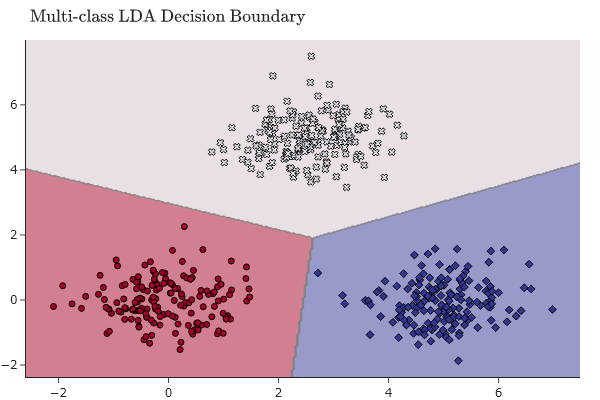
\includegraphics[width=0.6\textwidth]{chapters/classification/figures/lda_decision_boundary.png}
	\caption{\textbf{LDA Decision Boundaries} for a multiclass setup of three Gaussians. \GitChapterThreeExamples}
	\label{lda_decision_boundary}
\end{figure}

\paragraph{Learning A LDA Classifier}
So, in order to predict using an LDA classifier we need to know the class probabilities $\pi$, the means $\mu_0, \mu_1$ and the covariance matrix $\Sigma$. To do so we derive the maximum likelihood estimators. Given a training set $\trainset$ then the likelihood is given by:

$$
\begin{array}{ccl}
\mathcal{L}\left(\Theta|\X,\y\right) & = & \Prob\left(\left\{\left(\x_i,y_i\right)\right\}^m_{i=1}|\Theta\right)\\
& \overset{iid}{=} & \prod\Prob\left(\x_i,y_i|\Theta\right)  \\
& = & \prod\Prob\left(\x_i|y_i\right)\Prob\left(y_i|\Theta\right)\\
& = & \prod\pi_{y_i}\Nc\left(\x_i|\mu_{y_i},\Sigma\right)
\end{array}
$$

where $\Theta\coloneqq\left\{\pi,\mu_0,\mu_1,\Sigma\right\}$. By taking the derivative, each time with respect to $\pi$, $\mu_0$, $\mu_1$ and $\Sigma$ we find that the MLE are:
\begin{eqnarray}
\widehat{\pi}^{MLE}_y &\coloneqq &\frac{1}{m}\sum \indc{y_i = 1} = \frac{m_y}{m} \\
\widehat{\mu_y}^{MLE} &\coloneqq &\frac{1}{m_y}\sum \indc{y_i=y}\x_i \\
\widehat{\Sigma}^{MLE} &\coloneqq &\frac{1}{m} \sum_y \sum_{i:y_i=y}\left(\x_i-\widehat{\mu}_{y_i}^{MLE}\right)\left(\x_i-\widehat{\mu}_{y_i}^{MLE}\right)^\top \label{cov_mle}
\end{eqnarray}

for $m_y, \,\,y\in\left\{0,1\right\}$ denoting the number of samples seen each of the classes. Looking closely at the expressions derived we in fact realize that the MLE predicts the values proportional to what is found in the training set.

\begin{remark}
The covariance estimator described in \ref{cov_mle} is the one derived when equating the derivative with respect to $\Sigma$ to zero. This is a \textit{biased} estimator. The unbiased estimator for the covariance matrix is given by multiplying by $\frac{1}{m-2}$ instead of $\frac{1}{m}$:
$$ \widehat{\Sigma}^{MLE} \coloneqq \frac{1}{m-2} \sum_y \sum_{i:y_i=y}\left(\x_i-\widehat{\mu}_y^{MLE}\right)\left(\x_i-\widehat{\mu}_y^{MLE}\right)^\top$$
This covariance matrix expression is known as the \textit{pooled covariance} and it accounts for the use of an estimator of $\widehat{mu_j}$ rather the true parameter $\mu_j$. In the general case of multi-classification the multiplication factor of the unbiased estimator is $\frac{1}{m-K} $ where $K$ is the number of classes.
\end{remark}

\subsection{Quadratic Discriminant Analysis}
In the LDA algorithm we assumed the data is generated from a set of Gaussians, differing in their mean but sharing the same covariance matrix (\ref{lda_generative}). The Quadratic Discriminant Analysis algorithm allows different covariance matrices. That is, for any $i\in 1,\ldots,m$ we assume that:
\begin{equation}\label{qda_generative}
	\begin{array}{c}
		y_i \sim Ber\left(\pi\right) \\
		x_i|y_i \sim \Nc\left(\mu_{y_i},\Sigma_{y_i}\right)
	\end{array}
\end{equation}

~\\By enabling different covariance matrices the quadratic expression (in $\x$) of $\Prob\left(y=k|\x\right)$ does not cancel out. This in turn causes the decision boundaries between classes to be quadratic rather than linear. In both \autoref{lda_decision_boundary} and \autoref{qda_decision_boundary} the same data was used to fit either the LDA or the QDA models. We can see that while the decision boundaries of the LDA fit (\autoref{lda_decision_boundary}) are linear, in the case of QDA (\autoref{qda_decision_boundary}) we get curved (quadratic) boundaries.

\begin{figure}[h!]
	\centering
	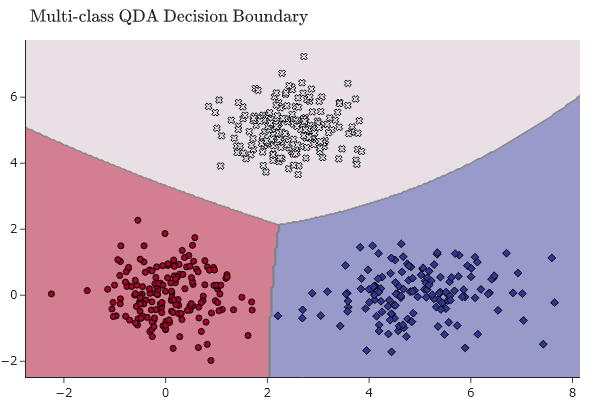
\includegraphics[width=0.6\textwidth]{chapters/classification/figures/qda_decision_boundary.png}
	\caption{\textbf{QDA Decision Boundaries} for a multiclass setup of three Gaussians. \GitChapterThreeExamples}
	\label{qda_decision_boundary}
\end{figure}

\paragraph{Learning A QDA Classifier}
Fitting a QDA classifier is very similar to the process of fitting a LDA classifier. The difference is in the estimation of the covariance matrices. In this case we fit a different covariance matrix for each class based on the samples of the class:

\begin{equation}
\widehat{\Sigma}^{MLE}_y \coloneqq \frac{1}{m_y} \sum_{i:y_i=y}\left(\x_i-\widehat{\mu}_{y}^{MLE}\right)\left(\x_i-\widehat{\mu}_{y}^{MLE}\right)^\top \label{cov_mle}
\end{equation}

\section{Nearest Neighbors}
Nearest Neighbors learners predict the label of a new sample based on a set of "nearset" training samples. This means that it has no hypothesis class and no training stage per se. As prediction is based on some subset of training samples, that is determined by "closeness" to some newly given sample, the training step of the learner consists only of storing the training data so it is available for the learner when performing predictions.

~\\This family of leaners are part of a wider \textbf{graph-based approach} for learning. In this approach we first define some graph structure over the samples - forming the nodes of the graph. Then, using the constructed graph we perform training and prediction. The different learners differ in how to define edges in the graph? are they weighted or not? how to transition between nodes? and how is this structure used for training and prediction?

\subsection{Prediction Using $k$-NN}
Let us begin with the simplest form of $k$-NN: given a training set \trainset and some distance function $\rho:\R^d\times\R^d\rightarrow\R_+$, prediction for a new sample $\x'$ is done by:
\begin{itemize}
	\item Compute distance from $\x'$ with respect to $\rho$: $\forall\, \x\in S\quad d_{\x}\coloneqq \rho\left(\x',\x\right)$.
	\item Denote $\pi=\left(\pi_1,\ldots,\pi_m\right)$ the permutation of $\left(1,\ldots,m\right)$ such that $d_{\x_{\pi_{1}}}\leq \ldots \leq d_{\x_{\pi_{m}}}$
	\item Select $k$ nearest samples $\x_{\pi_{1}},\ldots,\x_{\pi_k}$ and predict by majority vote: $$ \widehat{y}=\underset{y\in\left\{0,1\right\}}{argmax}\sum^k_{i=1}\mathbbm{1}\left[y_{\pi_i}=y\right] $$ 
\end{itemize}

\subsection{Computational Implementation}
Implementing a $k$-nearest-neighbors classifier is very easy on small datasets, but becomes computationally challenging (either in terms of execution time or in terms of space) when $d$ and/or $m$ are large. There are generally three types of implementation approaches:
~\\\begin{itemize}
	\item \textbf{Brute force implementation:} We keep the entire training sample $S$ in storage during the entire prediction process. For each new test sample $\x\in\R^d$ we calculate $\rho\left(\x,\x_i\right)\,\,i\in\left[m\right]$ and partially sort to find the $k$ smallest distances.  
	
	Suppose $\rho$ is the Euclidean distance. What are the computational costs of prediction? As the sample space is $\R^d$ computing the distance between two points is $\mathcal{O}\left(d\right)$. Doing so for all points in the dataset is $\mathcal{O}\left(dm\right)$. Next we want to retrieve the $k$ nearest train samples. If $k\ll m$ we can retrieve $k$ times the sample of minimal distance (without repeating previously selected samples) in a time complexity of $\mathcal{O}\left(km\right)$. However, if $k\approx ....$ then it is more computationally efficient to sort all distances and then select the $k$ minimal. Lastly, summation over selected samples is done in $\mathcal{O}\left(k\right)$. All together the time complexity of such approach is $\mathcal{O}\left(dm+km\right)$. In terms of space complexity we must store distances of all training samples and thus $\mathcal{O}\left(m\right)$.
	~\\\item \textbf{Exact nearest neighbors search with preprocessed data structure:} Depending on the selection of $\rho$, we could pre-process the training sample and construct a special data structure. After doing so in the training step, we can use this data structure to quickly locate the $k$ nearest neighbors of a given test sample. In the case of $\rho$ being the Euclidean distance we could you an algorithm such as \textit{kd-tree}.
	~\\\item \textbf{Fast randomized nearest neighbors search:} Beyond the scope of this course. \todo{add a single explanation sentence - or remove bullet all together}
\end{itemize}

\subsection{Selecting Value of $k$ Hyper-Parameter}
A very important aspect in $k$-NN is the chosen value of $k$. Though methods for determining the "right" $k$ will be discussed in future chapters, let us dwell on a few cases:
\begin{itemize}
	\item \textbf{$k=1$:} The test point is given the label of the single nearest neighbor in the training set. Such classifier has a very low bias but very high variances.
	\item \textbf{$k=m$:} The classifier predicts a single label for any given test sample, regardless to its values. It will predict the majority vote of the training set labels. In this case the bias is very high and the variance is zero.
\end{itemize}

\todo{Add 3 decision boundaries of 1,k,m-NN classifiers}

As we change $k$ we change the bias-variance tradeoff. 

\todo{KNN - misclassification as function of $k$}


\section{Decision Trees}
Decision Trees are classification and regression methods by which we partition the sample space into disjoint parts. Then, given such a partition, the response of our classification (or regression) is computed based on the training samples in the partition of the observation in question. These methods are very intuitive and yet capture many interesting aspects of learning. We will discuss some of these aspects in details in the following chapter.

\begin{remark}
	To this day, one of the more powerful classification and regression algorithms is what is called: Classification And Regression Trees (CART) Random Forest. It uses the power of committee decisions over the basic decision trees to achieve very good performances. Some of the aspects of this algorithm will be discussed in later chapters.
\end{remark}

\subsection{Axis-Parallel Partitioning of $\R^d$}
Earlier in this chapter we have discussed two classifiers that use piecewise-constant prediction rules: half-spaces and SVM. For noth, the hypothesis class consisted of half-spaces where prediction was determined by position of sample with respect to the hyper-plane. For decision trees we will describe a more complicated piecewise-constant prediction rule (more complex hypotheses). Let us consider a rule that partitions the sample space $\R^d$ into \textbf{axis-parallel boxes, or "hyper-rectangles"} where each box is associated with labels $1$ or $-1$. The learner's task would be to use the training sample to "chop" the samples space $\Xc$ int a disjoint union of axis-parallel boxes, and to assign a class prediction to each box.

\begin{figure}[h!]
	\centering
	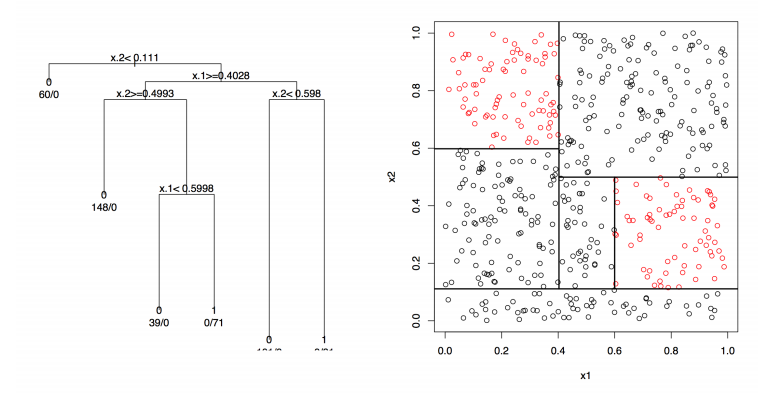
\includegraphics[width=0.7\textwidth]{chapters/classification/figures/decision_tree.png}
	\caption{Decision tree and induced partitioning of $\R^2$ sample space}
\end{figure}

To make out hypothesis $\Hc_{CT}$ class smaller and simpler, we will focus on disjoint unions of boxes that are obtained by iteratively splitting an existing box into two smaller boxes along one of the axes:
\begin{itemize}
	\item We start with the whole sample space $\R^d$.
	\item By selecting some coordinate $i_1\in \left[d\right]$ and some value $t_1\in\R$ we split $R^d$ into two axis-parallel "boxes" (half-spaces). We obtain: $$ B_1^+=\left\{\x\in\R^d|\x_{i_1}>t_1\right\},\quad B_1^{-}=\left\{\x\in\R^d|\x_{i_1}\leq t_i\right\} $$ 
	\item Next, by focusing of some previously split "box" $B_j^s$ for $s\in\left\{-,+\right\}$, we can again select some coordinate $i_{j+1}\in\left[d\right]$ and some splitting value $t_{j+1}\in\R^d$ to obtain $B_{j+1}^{-}, B_{j+1}^{+}$. Notice that $B_{j+1}^{-}$ and $B_{j+1}^{+}$ are disjoint, and if following this procedure then by induction they are also disjoint from any other obtained box.
\end{itemize}

Note that the partitions obtained this way are special - most partitions of $\R^d$ into axis-aligned boxes are not Tree Partitions. Namely, cannot be constructed by such a top-down iterative chopping procedure.
\begin{figure}[h!]
	\centering
	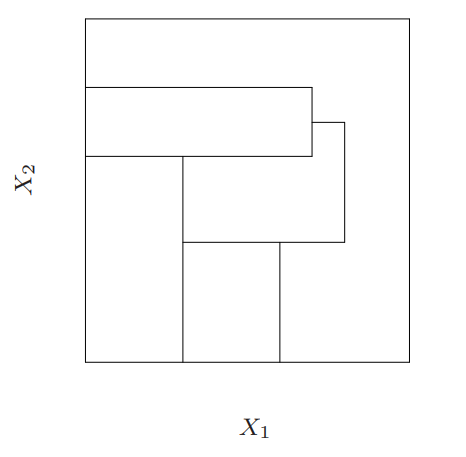
\includegraphics[width=0.4\textwidth]{chapters/classification/figures/axis_parallel_partition.png}
	\caption{Partitioning $\R^2$ into axis-aligned boxes not describing a tree partition}
\end{figure}

\subsection{Classification \& Regression Trees}
The hypothesis class $\Hc_{CT}$  we will consider consists of piecewise-constant functions, that assign a class prediction (1 or 0) to each box in a Tree Partition. Unless we restrict it somehow, the class contains all piecewise-constant functions supported on all Tree Partitions of $\R^d$ (to any number of boxes). Formally, for a Tree Partition $\R^d=\biguplus_{j=1}^N B_j$ of $\R^d$ into $N$ boxes, and label assignments $c_j \in \left\{ 0,1\right\}$ ($j=1,\ldots, N$) assigning label $c_j$ to box $B_j$, the hypothesis $h\in\Hc_{CT}$ is a function $h:\R^d\to\left\{ 0,1 \right\}$ defined by $$ h(\x) = \sum_{j=1}^N c_j \mathbbm{1}_{B_j}(\x) $$ where $\mathbbm{1}_{B_j}$ is the indicator function of $B_j$. 

\begin{example}
	Consider the following scenario: suppose someone comes into a hispital emergency room. The first step of triage is to determine - fast - whether they are in a life-threatening medical emergency, or else they can wait in line and receive treatment in a little while. The triage uses a sequence of yes/no questions, such as: Is the patient conscious yes/no?
	\begin{itemize}
		\item If not conscious: classify as \textbf{emergency}
		\item If patient is conscious: is the patient's pulse $<40$ beats per minute?
		\begin{itemize}
			\item If yes (pulse $<40$): classify as textbf{emergency}
			\item If no, (pulse $\geq 40$): is the patient's pulse $>130$ beats per minute?
			\begin{itemize}
				\item If yes (pulse $>130$): is the patient's systolic blood pressure $<80$ mmHg?
				\begin{itemize} %TODO - allow deeper levels
					\item If yes classify as \textbf{emergency}
					\item If not, is the patient's systolic blood pressure $>140$ mmHg? If yes, classify as \textbf{emergency}. Otherwise, classify as \textbf{no emergency}
				\end{itemize}
				\item If not classify as \textbf{no emergency}
			\end{itemize}
		\end{itemize}
	\end{itemize}
	
	~\\This is a decision tree that uses three features: conscious (a binary categorical feature), pulse (a numerical feature) and blood pressure (also a numerical feature). See if you can we write a diagram for this decision tree in the shape of a tree, where every node is a question, and every leaf is a decision / classification. The root of the tree is the first question ("conscious yes/no?").
	Now observe that every function in our Classification Trees hypothesis class $\Hc_{CT}$ is equivalent to a decision tree. In the notations of the generic example above, the first question is: "$x_{i_1}>t_1$-yes/no?".  If yes, we ask the second question "$x_{i_{2,1}}>t_{2,1}$ - yes/no?". If not, we ask the second question: "$x_{i_{2,2}}>t_{2,2}$ - yes/no?". And so on, until there are no more splits and we have reached a box over which the function in $\Hc_{CT}$ is constant. If the constant value is $1$, we classify / predict class $1$. If the constant value is $0$, we predict class $0$. This is why our hypothesis class is called - classification trees
\end{example}

\subsection{Growing a Classification Tree}
Having defined our hypothesis class, the next question is of course what learning principle shall we use. That is, how shall be select $h_s\in\Hc_{CT}$ based on the training sample $S$. Suppose we have already obtained a Tree Partition of $\R^d$ is some manner, that consists of $N$ disjoint boxes $\R^d=\biguplus_{j=1}^{N}B_j$. Let $\trainset$ be our taining set and denote the predicted label assigned to box $B_j$ by $\widehat{y}\left(B_j\right)\in\left\{0,1\right\}$. As such, the number of mis-classification errors that are incurred by the training sample that fall inside $B_j$ is $\sum_{\x_i\in B_j}\mathbbm{1}\left[y_i\neq\widehat{y}\left(B_j\right)\right]$.

Let us begin learning by applying the ERM principle. Denote the fraction of correctly classified samples with label $y\in\left\{0,1\right\}$ in some box $B$ by:
$$ P^S_y\left(B\right)\coloneqq \frac{1}{n_S\left(B\right)}\sum_{\x_i\in B}\mathbbm{1}\left[y_i=y\right]  $$ where $n_S\left(B\right)$ is the number of training samples that fall inside the box $B$. The label that will minimize the empirical risk for those training samples in box $B$ is the \textbf{majority vote} over the labels. So, for any sample falling in box $B$ we would predict $$ \widehat{y}_S\left(B\right)=\underset{y\in\left\{0,1\right\}}{argmax}P^S_y\left(B\right) $$
Applying over the entire Tree Partition, minimizing the empirical risk is achieved by labeling box $B_j$ with $\widehat{y}_S\left(B_j\right),\quad  j\in\left[N\right]$. Therefore, for a given training set $S$, every Tree Partition corresponds with a unique label assignment, and as such, a unique classification tree $h\in\Hc_{CT}$ that minimizes the empirical risk. It seems therefore, that finding the desired ERM tree is done by solving $$ \underset{h\in\Hc_{CT}}{argmin}L_S\left(h\right) $$ where $L_S\left(h\right)$ is the misclassification error of $h$ over $S$.

~\\Looking back at the described procedure could you describe which tree would minimize the empirical risk and therefore be selected (for any training set $S$)? Consider the tree where the number of leaves is $\left|S\right|$ and each sample is in a box containing only itself. Following the prediction rule we devised, such a tree would achieve $L_S\left(h\right)=0$. Though we achieved the lowest possible empirical risk, this tree will fail to generalize to new samples. To cope with this problem we should limit the number of levels in the classification tree (equivalent for limiting number of leaves). Denote $\Hc_{CT}^k$ the hypothesis class of all tree partitions with at most $k$ levels. Now, we will choose $k$ and then using the ERM principle return $$ \underset{h\in\Hc_{CT}^k}{argmin} L_S\left(h\right)$$

\paragraph{Selecting A Value For $k$:} Note that by adding the hyper-parameter $k$ we now have \textbf{a family of hypothesis classes}, one for each value of $k$. The value of $k$ controls the size of the hypothesis class and therefore controls the bias-variance tradeoff:
\begin{itemize}
	\item For small values of $k$, the hypothesis class is smaller, containing trees of smaller sizes. Therefore the ERM learner will have a \textbf{higher} bias as it can only select simple Tree Partitions. It will also have a \textbf{lower} variance: as the boxes are very large, the labels assigned to each box are based on a majority vote of typically many training samples. Therefore changing a few training samples will barely change the selected hypothesis.
	\item For large values of $k$, the hypothesis class is much more complex, with more "specialized" trees in it. Therefore the ERM learner will have a \textbf{lower} bias and \textbf{higher} variance.
\end{itemize}
Later in the course we will introduce a few methods for selecting the value of $k$.

\subsection{CART Heuristic For Growing Trees}
The next challenge is how to find the minimizer of $argmin_{h\in\Hc_{CT}^k} L_S\left(h\right)$ computationally? So far, all the ERM learners we encountered were \textbf{computationally tractable}: 
\begin{itemize}
	\item The linear regression optimization problem was based on ERM. We were able to find aclosed form expression for the minimizer.
	\item The Half-space classifier was based on ERM and lead to a simple convex optimization problem.
\end{itemize}

In contrast to those examples the search space over $\Hc_{CT}^k$ is exponentially large and has no Euclidean or other structure to be used. Finding an ERM solution would mean to use brute-force search, which is infeasible. In fact, it has been proven that implementing ERM on $\Hc_{CT}^k$ is an NP-Hard problem with respect to the training sample size\footnote{By reduction from "three dimensional matching", see Hyafil and Rovest, "Constructing Optimal Binary Decision Trees is NP-Complete", Information Processing Letters 5(1), 1976} .

~\\This is our first encounter with the bitter truth that though the ERM principle is nice, it is often impossible to implement efficiently, especially when the hypothesis class has no Euclidean structure. Therefore, we must resort to defining and using \textbf{heuristics}: an approach to solving the optimization problem that does not guaranteed to be optimal, but is still sufficient for finding a solution. While the definition of decision trees, the hypothesis class and prediction assignment to boxes in a tree partition are all canonical, there are several different heuristic approaches to the way we "grow a decision tree', namely to the way we choose an hypothesis in practice.

~\\One common approach, coming out of the statistical learning community, is called \textbf{Classification and Regression Trees} (CART). This heuristic cinsists of two stages: \textbf{growing} the tree, resulting in a tree that is a little too large, and then \textbf{pruning} it to bring it down to the most effective size.

Suppose we have chosen $k$ to be the maximal tree depth. The heuristic of growing a full decision tree with at most $k$ levels will proceed top-down, starting from $\R^d$ and progressively chopping each box into two boxes. A given box is \textbf{not chopped} if either:
\begin{itemize}
	\item The maximum number of levels $k$ has been reached.
	\item The box has reached a pre-determined minimal number of training samples. At the very least we would not split a box if it consists of only a single training sample.
\end{itemize}

Chopping is done by finding the \textbf{best} coordinate, at the \textbf{best} value to chop, and whenever you chop given each half-box the \textbf{best} class assignment, in the sense of minimizing misclassification error over the training sample.

~\\Formally, let $B$ be some box in an existing disjoint partitioning of $\R^d$ (at the very beginning this box is the entire sample space). Splitting $B$ is done as follows:
\begin{itemize}
	\item For each coordinate $i\in \left[d\right]$ and each potential chopping value $t\in\R$ we define $g_i\left(t\right)$ by:
	\begin{itemize}
		\item For each $t\in\R$ let us define the two boxes obtained from $B$ by splitting along coordinate $i$ at value $t$: $$ B^+_t\coloneqq \left\{\x\in\R^d|\x_i>t\right\},\quad B^-_t \coloneqq \left\{\x\in\R^d|\x_i\leq t\right\} $$
		\item Denote $\widehat{y}_S\left(B^{\pm}_t\right)$ be  the class assignment for boxes $B^{\pm}_t$ as defined above, minimizing the empirical misclassification risk in that box.
		\item Denote $P^S_{\widehat{y}_S\left(B^{\pm}_t\right)}\left(B^{\pm}_{t}\right)$ be the optimal empirical misclassification risk incurred by these class assignments.
		\item Now, let $g_i\left(t\right)$ be the best empirical risk incurred by chopping box $B$ at value $t$ along coordinate $i$: $$ g_i\left(t\right) \coloneqq  P^S_{\widehat{y}_S\left(B^{-}_t\right)}\left(B^{-}_{t}\right) + P^S_{\widehat{y}_S\left(B^{+}_t\right)}\left(B^{+}_{t}\right) $$ 
	\end{itemize}
	\item Denote $t_i$ to be the \textbf{best} chopping point along coordinate $i$ and calculate it for every coordinate: $$ t_i\coloneqq \underset{t\in\R}{argmin}g_i\left(t\right)\quad i=1,\ldots,d $$
	\item Let $i^{*}$ denote the \textbf{best} coordinate along which to chop $B$: $$ i^{*}\coloneqq \underset{i\in\left[d\right]}{argmin}g_i\left(t_i\right) $$
	\item Chop $B$ along coordinate $i^{*}$  at value $t_{i^{*}}$.
\end{itemize}

\paragraph{Time Complexity Analysis}
Before we introduced the CART heuristic we described that solving the ERM principle over this hypothesis class is NP-Complete and therefore cannot be done in polynomial time. Let us see that the CAR heuristic can indeed be computed efficiently. 

~\\The algorithm iteratively splits boxes into two by finding a coordinate $i\in\left[d\right]$ and a value $t\in\R$. It scans all $d$ coordinates and for each scans all possible values of $t$. Notice, that even though $t\in\R$ we do not need to try all values and it suffices to check only the values in the $i$'th coordinate of the training sample: $\left\{\x_i | \x\in S\right\}$. As we have $m$ samples we only need to evaluate for at most $m$ values, giving each step a time complexity of $\mathcal{O}\left(md\right)$.

~\\The next question is how many steps will the algorithm perform? We know that the algorithm will terminate after growing a tree with at most $k$ levels. Such a tree will have at most $2^k-1$ nodes and leaves. Though this seems exponentinal in the given input (notice that the hyper-parameter $k$ is also part of the input) we can upper bound this value. As we do not allow empty boxes (and in fact any box with less than some minimal number of samples) the number of nodes (including leaves) in the tree is at most $m$. We therefore conclude that the time complexity of the CART heuristic is $\mathcal{O}\left(m^2 d\right)$
\subsection{Pruning a Decision Tree}
\todo{Add explanation about pruning}
